\documentclass{article}
\usepackage{forest,ctex,amsmath,color,xcolor,colortbl,graphicx,geometry,comment,listings,hyperref,booktabs,tabularx,wrapfig,caption,calc,mhchem,fix-cm,tocloft,titlesec,setspace,fancyhdr,booktabs,float,subcaption,enumitem}
\usepackage{lastpage}
\usepackage[absolute,overlay]{textpos}  % 绝对定位
\setlength{\parindent}{2em} 
% ========== 标题格式定制(titlesec宏包) ========== %
\renewcommand{\thesection}{\chinese{section}}  % 一级标题编号:第X章
\renewcommand{\thesubsection}{\arabic{section}.\arabic{subsection}} % 二级:1.1
\renewcommand{\thesubsubsection}{\arabic{section}.\arabic{subsection}.\arabic{subsubsection}} % 三级:1.1.1
% 一级标题:三号黑体,居中,上下各空12pt(≈1行)
\titleformat{\section}
  [block]                  % 标题格式:display(带上下间距)
  {\centering \zihao{3} \heiti}  % 居中,三号黑体
  {\Large \thesection}       % 编号格式(Large字号,如“第一章”)
  {12pt}                     % 编号与标题的间距
  {}                         % 标题内容(无额外格式)
\titlespacing{\section}{0pt}{30pt}{30pt}  % 上间距12pt,下间距12pt

% 二级标题:四号黑体,缩进,编号显示(如“1.1”)
\titleformat{\subsection}
  {\zihao{4} \heiti}         % 四号黑体
  {\thesubsection}           % 编号(如“1.1”)
  {1em}                      % 编号与标题的间距
  {}
\titlespacing{\subsection}{0em}{1.5ex plus .5ex}{1ex plus .2ex}  % 左缩进2em

% 三级标题:小四号黑体,缩进,编号显示(如“1.1.1”)
\titleformat{\subsubsection}
  {\zihao{-4}}        % 小四号黑体(\zihao{-4}对应小四号)
  {\thesubsubsection}        % 编号(如“1.1.1”)
  {1em}                      % 编号与标题的间距
  {}
\titlespacing{\subsubsection}{0em}{1.5ex plus .5ex}{1ex plus .2ex}  % 左缩进2em


\geometry{left=2.5cm,right=2.5cm,top=2.5cm,bottom=2.5cm}
%\setlength{\parindent}{2pt} 
\date{}
\begin{document}
\vspace{-30pt}
\begin{center}
    \Large \textbf{数学建模比赛}  % 原字体可能是\Large,改为\large缩小
\end{center}
% 标题与“摘要”之间减少空白
\vspace{-13pt}
\begin{center}
    \large \textbf{摘要}  % 原字体可能是\large,改为\normalsize缩小
\end{center}
\qquad 本文针对NIPT(无创产前检测)技术中最佳检测时点选择与胎儿异常判定的问题,通过建立数学模型,对
孕妇进行合理分组并确定最佳检测策略,以最小化潜在风险并提高检测准确性。我们综合利用了数理统计等方法,
系统地解决了题目提出的四个问题。

针对问题一,本文首先进行了数据探索与预处理,通过散点图初步发现Y浓度随孕周呈上升趋势,与BMI的关
系则需进一步建模验证。为解决个体重复测量数据中的组内相关性并准确捕捉变量间潜在的非线性关系,我
们分别建立了\textbf{线性混合模型(LMM)}、\textbf{非线性混合模型(NLME)}和\textbf{广义可加混合模型(GAMM)}。综合比较表
明,GAMM具有最优的拟合性能能同时识别孕周和BMI的显著非线性影响,并验证了个体间存在显著差异。最
终基于GAMM得出结论:Y染色体浓度随孕周呈非线性增长,而与BMI之间存在复杂的非线性负相关关系,为
该类数据的分析提供了稳健的建模框架。

针对问题二,本研究基于临床已知的男胎孕妇BMI是影响胎儿Y染色体浓度达标时间的主要因素,
通过对孕妇BMI进行科学分组并确定最佳NIPT检测时点,以最小化孕妇潜在风险。首先,我们依据Y染色体浓度
达标情况将孕妇分为三组:始终达标组、中间达标组和从不达标组;接着采用\textbf{K-means聚类算法}对孕妇平均BMI
进行聚类分析,通过\textbf{肘部法则}确定最佳聚类数为5类;然后计算每个BMI区间的Y染色体浓度达标时间,以中位数
确定该组最佳检测时点;最后通过\textbf{误差传播模型}分析检测误差对结果的影响。结果表明,基于BMI分组的个性化
检测时点推荐能够有效降低临床风险,为NIPT临床实践提供了科学依据。

针对问题三

针对问题四

\textbf{关键词:线性混合模型,非线性混合模型,广义可加混合模型,K-means聚类算法,肘部法则,误差传播模型}
\newpage
\section{\textbf{问题重述}}
\subsection{\textbf{问题背景}}
NIPT(Non-invasive Prenatal Testing,无创产前检测)作为一项革命性的产前筛查技术,通过采集孕
妇外周血中的胎儿游离DNA进行测序分析,能够有效评估胎儿常见染色体非整倍体异常的风险[1]。该技术具
有无创、安全、准确性高等特点,已成为临床产前筛查的重要手段。

在实际临床应用中,NIPT检测的准确性受到多种因素影响,其中胎儿游离DNA浓度(特别是Y染色体浓度对
于男胎)是关键因素之一。临床实践表明,胎儿Y染色体浓度与孕妇孕周数及身体质量指数(BMI)存在显著
相关性。同时,检测时机的选择对于尽早发现胎儿异常、降低临床风险至关重要:早期发现(12周以内
)风险较低,中期发现(13-27周)风险较高,而晚期发现(28周以后)风险极高。

目前临床通常根据孕妇BMI值进行简单分组并确定统一的检测时点,但这种方法未能充分考虑孕妇年龄、体
重等个体差异,可能导致部分孕妇错过最佳检测时机,增加临床风险。因此,需要建立更加科学、个性化的
NIPT时点选择模型,为不同特征的孕妇群体制定最优检测策略。

\subsection{\textbf{问题要求}}
附件提供了某地区(大多为高BMI)孕妇的NIPT检测数据,包括孕妇年龄、BMI、孕周数、胎儿染色体浓度、
Z值、GC含量、读段数等相关指标。现需要根据这些数据建立数学模型,解决以下问题:

\textbf{问题一:}基于附件中的数据,分析胎儿Y染色体浓度与孕妇孕周数、BMI等指标的相关特性,建
立合适的数学模型描述它们之间的关系,并对模型的显著性进行统计检验。

\textbf{问题二:}临床证明男胎孕妇的BMI是影响胎儿Y染色体浓度达标时间(浓度≥4\%的最早时间)的
主要因素。请对男胎孕妇的BMI进行合理分组,确定每组的BMI区间和最佳NIPT检测时点,使得孕妇的潜在
风险最小,并分析检测误差对结果的影响。

\textbf{问题三:}综合考虑体重、年龄等多种因素对男胎Y染色体浓度达标时间的影响,同时考虑检测误
差和胎儿Y染色体浓度达标比例,根据男胎孕妇的BMI进行合理分组,确定每组的最佳NIPT检测时点,使孕
妇潜在风险最小,并分析检测误差对结果的影响。

\textbf{问题四:}针对女胎异常的判定问题,以女胎孕妇的21号、18号和13号染色体非整倍体为判定结
果,综合考虑X染色体及上述染色体的Z值、GC含量、读段数及相关比例、BMI等因素,建立女胎异常的判定
模型和方法。

\section{\textbf{问题分析}}
\subsection{\textbf{问题一的分析}}
问题一要求分析Y染色体浓度与孕周数、BMI之间的相关关系,由于数据来源于同一孕妇的多次检测,存在明
显的组内相关结构,传统回归方法无法处理该类数据且会导致估计偏差。同时,生物学背景表明孕周与浓度
间可能存在非线性增长模式,而BMI亦可能通过稀释效应产生非线性影响。因此,需采用能同时兼容个体随
机效应与变量非线性关系的混合建模策略。我们首先通过个体线性回归初步探索趋势,发现普遍正增长但存
在个体差异,且BMI与浓度增长率线性相关不明显,暗示简单线性假设不足。进而,分别建立LMM、NLME和
GAMM三类混合模型进行系统比较,最终依据GAMM显著的非线性识别能力和更高的拟合优度,选择其作为揭
示变量间复杂相关特性的核心模型。
\subsection{\textbf{问题二的分析}}
针对问题二,其要求根据男胎孕妇的BMI进行合理分组并确定最佳检测时点。我们根据Y染色体浓度是否达
标(≥4\%)将孕妇分为三类,反映不同孕妇的Y染色体浓度变化规律。然后采用K-means聚类算法对孕妇平均BMI
进行客观分组,避免主观划分的随意性。通过肘部法则确定最佳聚类数为5,确保了分组的科学性和合理性。
接着对于每个BMI分组,计算组内孕妇的Y染色体浓度达标时间(对于中间达标组采用插值法预测),以中位数
作为该组的最佳检测时点,减少异常值影响。最后考虑检测过程中可能存在的测量误差和模型误差,通过误差
传播模型评估这些误差对达标时间预测的影响程度,确保推荐时点的可靠性。
\subsection{\textbf{问题三的分析}}

\subsection{\textbf{问题四的分析}}

\section{\textbf{模型假设}}
1.假设附件所提供的孕妇NIPT检测数据真实、准确,且数据样本足以反映胎儿染色体浓度与孕妇孕周、BMI等指标间的统计规律。

2.假设题目中给出的Y染色体浓度4\% 的临界值是可靠且普适的。

3.假设具有相似特征(如处于同一BMI区间)的孕妇群体,其胎儿Y染色体浓度的增长规律和达标时间具有相似的统计特征。

4.假设题目所提供的特征(包括但不限于X、21、18、13号染色体的Z值、GC含量、读段数比例及孕妇BMI等)包含了足以有效判别女胎染色体是否异常的信息。
\section{\textbf{符号说明}}
\begin{table}[htbp]
    \centering
    % 列格式:第一列居中+固定宽3cm,第二列居中
    \begin{tabular*}{\linewidth}{@{\extracolsep{\fill}}>{\centering\arraybackslash}p{3cm} c}
        \toprule  % 顶部粗线
        符号 & 说明 \\
        \midrule  % 表头与内容间的细线
        $k_i^{(c)}$ & 孕妇代码为$i$的个体Y染色体浓度与孕周线性回归方程斜率 \\
        $k_i^{(b)}$ & 孕妇代码为$i$的个体BMI指数与孕周线性回归方程斜率  \\
        $Y_{ij}$ & 孕妇代码为$i$的个体第$j$次检测得到的Y染色体浓度\\
        $G_{ij}$ & 孕妇代码为$i$的个体第$j$次检测的检测孕周(天为单位)\\
        $BMI_i$ & 表示第$i$个孕妇的身体质量指数(常数对于每个孕妇)\\
        $\overline{b}$ & 所有孕妇个体BMI增长率的平均数\\
        \bottomrule  % 底部粗线
    \end{tabular*}
    \label{tab:symbols}
\end{table}
%%%%%%%%%%%%%%%%%%%%%%%%%%%%%%%%%%%%%%%%%%%%%%%%%%%%%%%%%%%%%%%%%%%%%%%%%%%%%%%%%%%%
%%%%%%%%%%%%%%%%%%%%%%%%%%%%%%%%%%%%%%%%%%%%%%%%%%%%%%%%%%%%%%%%%%%%%%%%%%%%%%%%%%%%
%                                   QUESTION ONE                                   %
%%%%%%%%%%%%%%%%%%%%%%%%%%%%%%%%%%%%%%%%%%%%%%%%%%%%%%%%%%%%%%%%%%%%%%%%%%%%%%%%%%%%
%%%%%%%%%%%%%%%%%%%%%%%%%%%%%%%%%%%%%%%%%%%%%%%%%%%%%%%%%%%%%%%%%%%%%%%%%%%%%%%%%%%%
\section{\textbf{问题一模型建立求解}}
\subsection{\textbf{模型建立思路}}
问题一要求分析胎儿Y染色体浓度与孕妇孕周数和BMI等指标的相关特性。我们先观察通过分析数据,对每个
人线性回归,发现了绝大多数人y和时间关系与y和增长率和BMI增长率关系,以此我们判定,所有曲线都遵
循一个共同的、内在的生物学规律,但由于个体差异,曲线的高度和形状会各不相同。为精确刻画个体增
长规律并避免群体平均带来的巨大偏差,我们决定采用基于个体时间序列的混合效应方法。核心思路是:首
先对数据进行筛选,保证每个个体的数据点数量足以支持回归分析,;然后通过使用三种线性与非线性混合效
应模型,比较得出最优是GAMM,并且根据这个得出得出胎儿Y染色体浓度与孕妇孕周数和BMI的相关特性。
\subsection{\textbf{数据预处理}}
为探究Y染色体浓度与孕妇孕周数和BMI的关系,我们分别以检测孕周(天数)和BMI为x轴,Y染色体浓度为y轴,
绘制了散点图(其中相同颜色的点代表同一个人),如下:
% 单个图片
\begin{figure}[H]  % [H]表示强制当前位置(可选参数:h=此处,t=顶部,b=底部,p=单独页)
    \centering  % 图片居中
    % 插入图片:width=0.8\textwidth 表示占页面宽度的80%(可调整)
    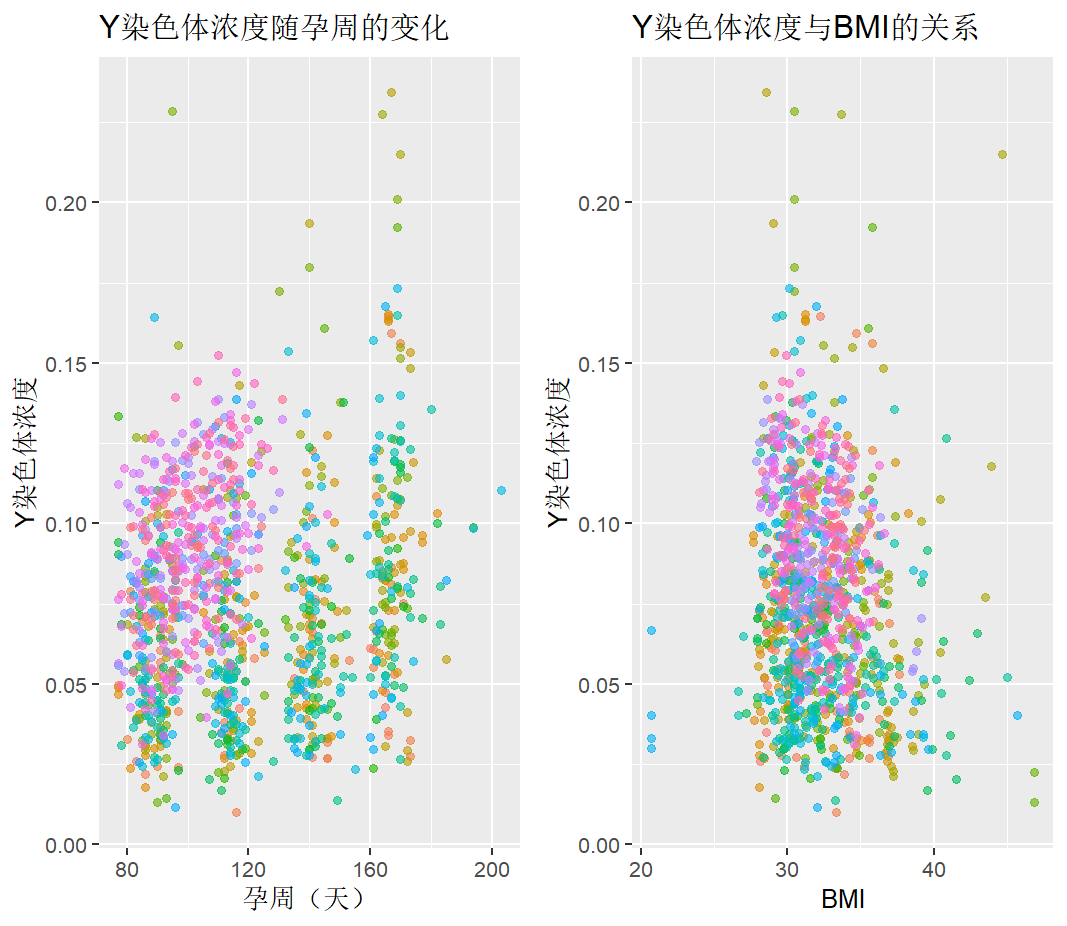
\includegraphics[width=0.7\textwidth]{graph/sss.png}  % 替换为实际图片路径
    \caption{y染色体浓度散点图}  % 图片标题
    \label{fig:single}  % 标签(用于交叉引用:\ref{fig:single})
\end{figure}
分析左图(Y染色体浓度随孕周变化)可见,随着孕周从80天增加到200天,Y染色体浓度整体呈上升趋势,
散点分布呈现明显的"向右上方扩散"特征。特别是在孕周大于160天后,高浓度点(Y$\geq$0.15)的出现频率
显著增加,这表明Y染色体浓度与孕周之间存在正相关关系

分析右图(Y染色体浓度与BMI关系)显示,随着BMI值在20-40范围内变化,Y染色体浓度的散点分布未呈现
明显的单向变化趋势。然而,结合后续模型得到的负系数估计值(c = -0.0042),提示Y染色体浓度可能
随BMI增加而轻微下降,但这种趋势在散点图中不够明显,可能需要通过模型来进一步验证。

需要注意的是,原始数据中存在个别孕妇检测次数过少的情况,这会导致回归结果不可靠。为确保模型稳定
性,我们设定了数据筛选条件:仅保留检测次数大于3次的孕妇数据。
\subsection{\textbf{线性回归模型}}
分析胎儿 Y 染色体浓度与孕妇的孕周数和 BMI 等指标的相关特性,本研究为每位孕妇建立了双变量时间
序列回归模型。从预处理后的有效数据中,筛选出每位孕妇多次检测的记录,分别建立以下两个一元线性
回归模型:

\textbf{1. Y染色体浓度-时间关系模型:}\\
以检测时间($t_{ij}$)为自变量,对应的Y染色体浓度($c_{ij}$)为因变量,建立回归模型:
\begin{gather}
    c_{ij}=k_i^{(c)}*t_{ij}+b_i^{(c)}+\epsilon_{ij}^{(c)} \tag{1}
\end{gather}

其中:$k_i^{(c)}$ 表示第 $i$ 位孕妇的胎儿Y染色体浓度的日增长率,这是我们关注的核心参数;
$b_i^{(c)}$ 为截距项;$\epsilon_{ij}^{(c)}$ 为随机误差项。

\textbf{2. BMI-时间关系模型:}\\
以检测时间($t_{ij}$)为自变量,对应的Y染色体浓度($c_{ij}$)为因变量,建立回归模型:
\begin{gather}
    c_{ij}=k_i^{(b)}*t_{ij}+b_i^{(b)}+\epsilon_{ij}^{(b)} \tag{2}
\end{gather}

我们采用最小二乘法进行参数估计,并计算确定系数 $R^2_i$ 以评估拟合优度
\subsection{\textbf{Y染色体浓度与时间关系的个体分析}}
基于建立的所有个体回归模型,我们首先对模型的关键参数进行了统计分析,结果如下表所示:
\begin{table}[htbp]
    \centering
    \begin{tabular*}{\linewidth}{@{\extracolsep{\fill}}c c c c}
        \toprule  % 顶部粗线
        统计量 & 斜率 $k_i$(\%/天) & 截距        & 确定系数$R_i^2$ \\
        \midrule  % 表头与内容间的细线
        平均值 & 0.000800       & -0.005467 & 0.861443    \\
        标准差 & 0.00316        & 0.038959  & 0.123487    \\
        最小值 & 0.001752       & 0.088208  & 0.999747    \\
        最大值 & 0.000205       & -0.151320 & 0.505933    \\
        \bottomrule  % 底部粗线
    \end{tabular*}
    \label{tab:crops_booktabs}
\end{table}

从表中可知,个体的Y染色体浓度均随孕天增加呈现明显的上升趋势,绝大部分模型的拟合优度较高(平均
$R^2=0.824$表明线性模型能够很好地描述浓度随时间变化的规律。
\subsection{\textbf{BMI增长率与Y染色体浓度增长率的全局相关性分析}}
为探究BMI是否导致了上述增长速率的差异,我们计算了每位孕妇的BMI增长率个体Y染色体浓度增长率 $k_i$ 的相关性。

我们绘制了标准化BMI增长速率与斜率 $k_i$ 在相应编号下的散点图
与两者在不同维度下绘制的图像,如下
%两个图并排
\begin{figure}[H]
    \centering
    % 子图1:宽度占页面的45%(左右留空)
    \begin{subfigure}[b]{0.45\textwidth}  % [b]表示底部对齐
        \centering
        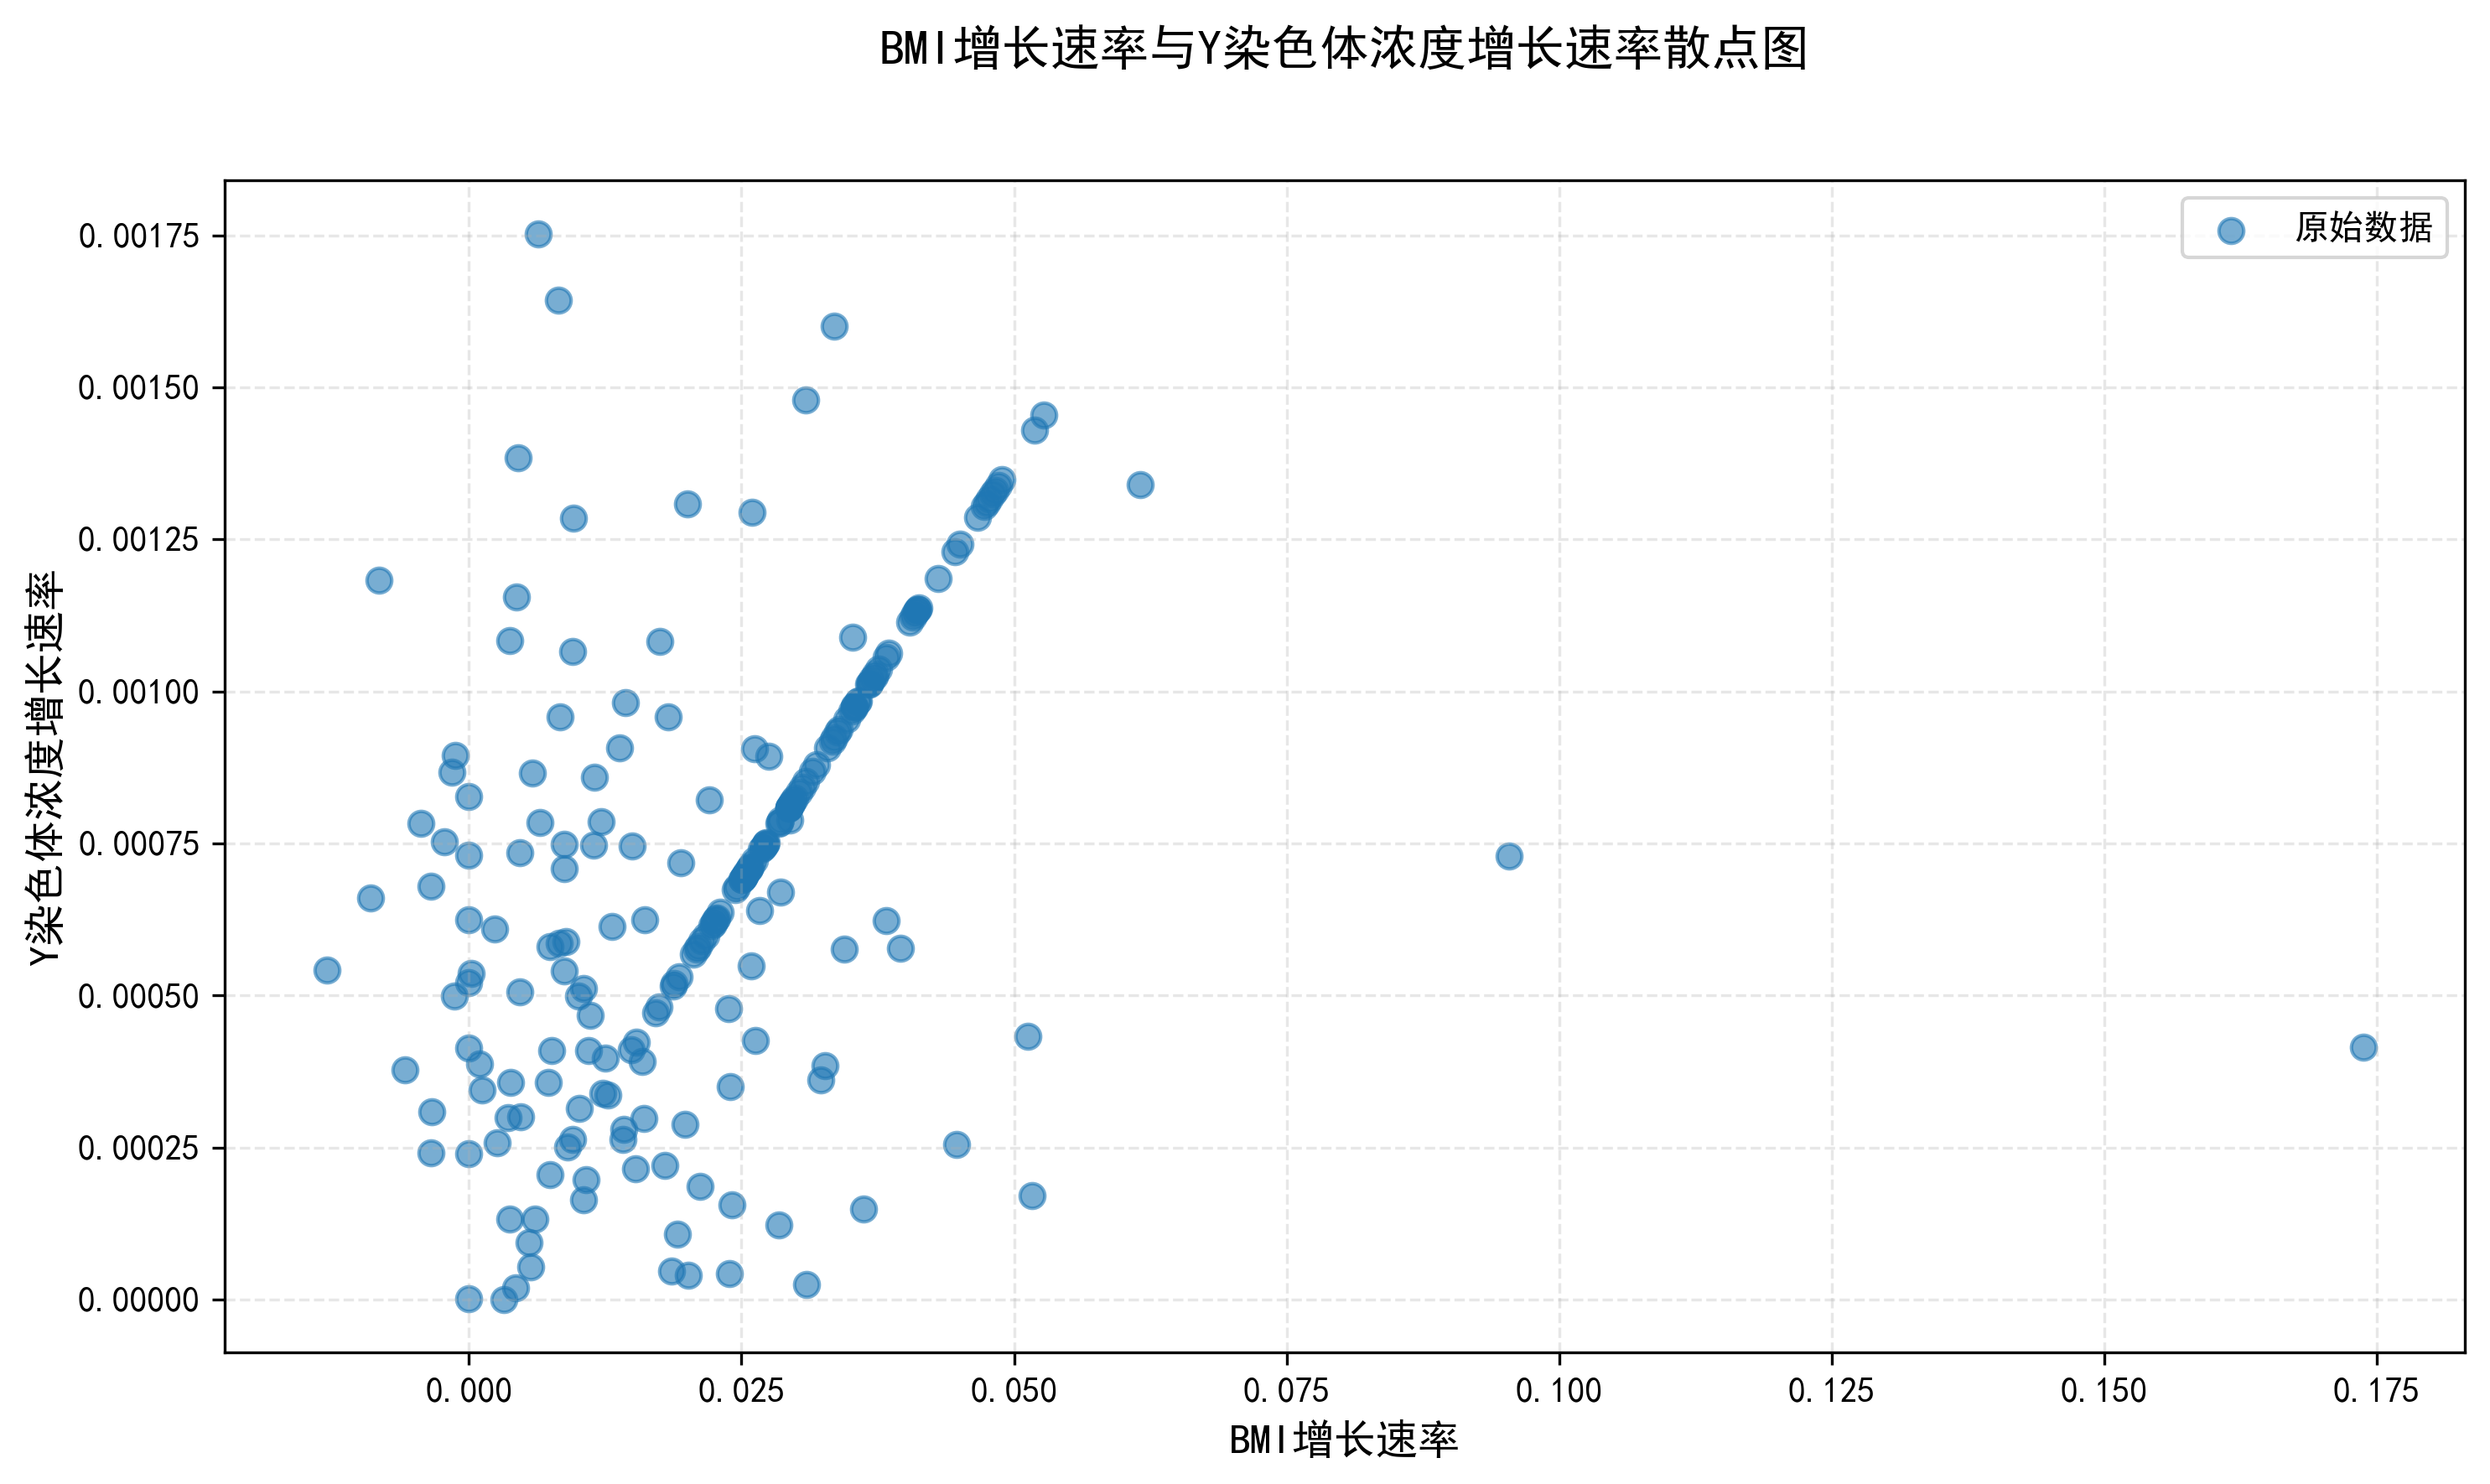
\includegraphics[width=\textwidth]{graph/points.png}  % 宽度=子图宽度
        \label{fig:sub1}  % 子图标签
    \end{subfigure}
    \hspace{0.05\textwidth}  % 两图间距(5%页面宽度)
    % 子图2
    \begin{subfigure}[b]{0.45\textwidth}
        \centering
        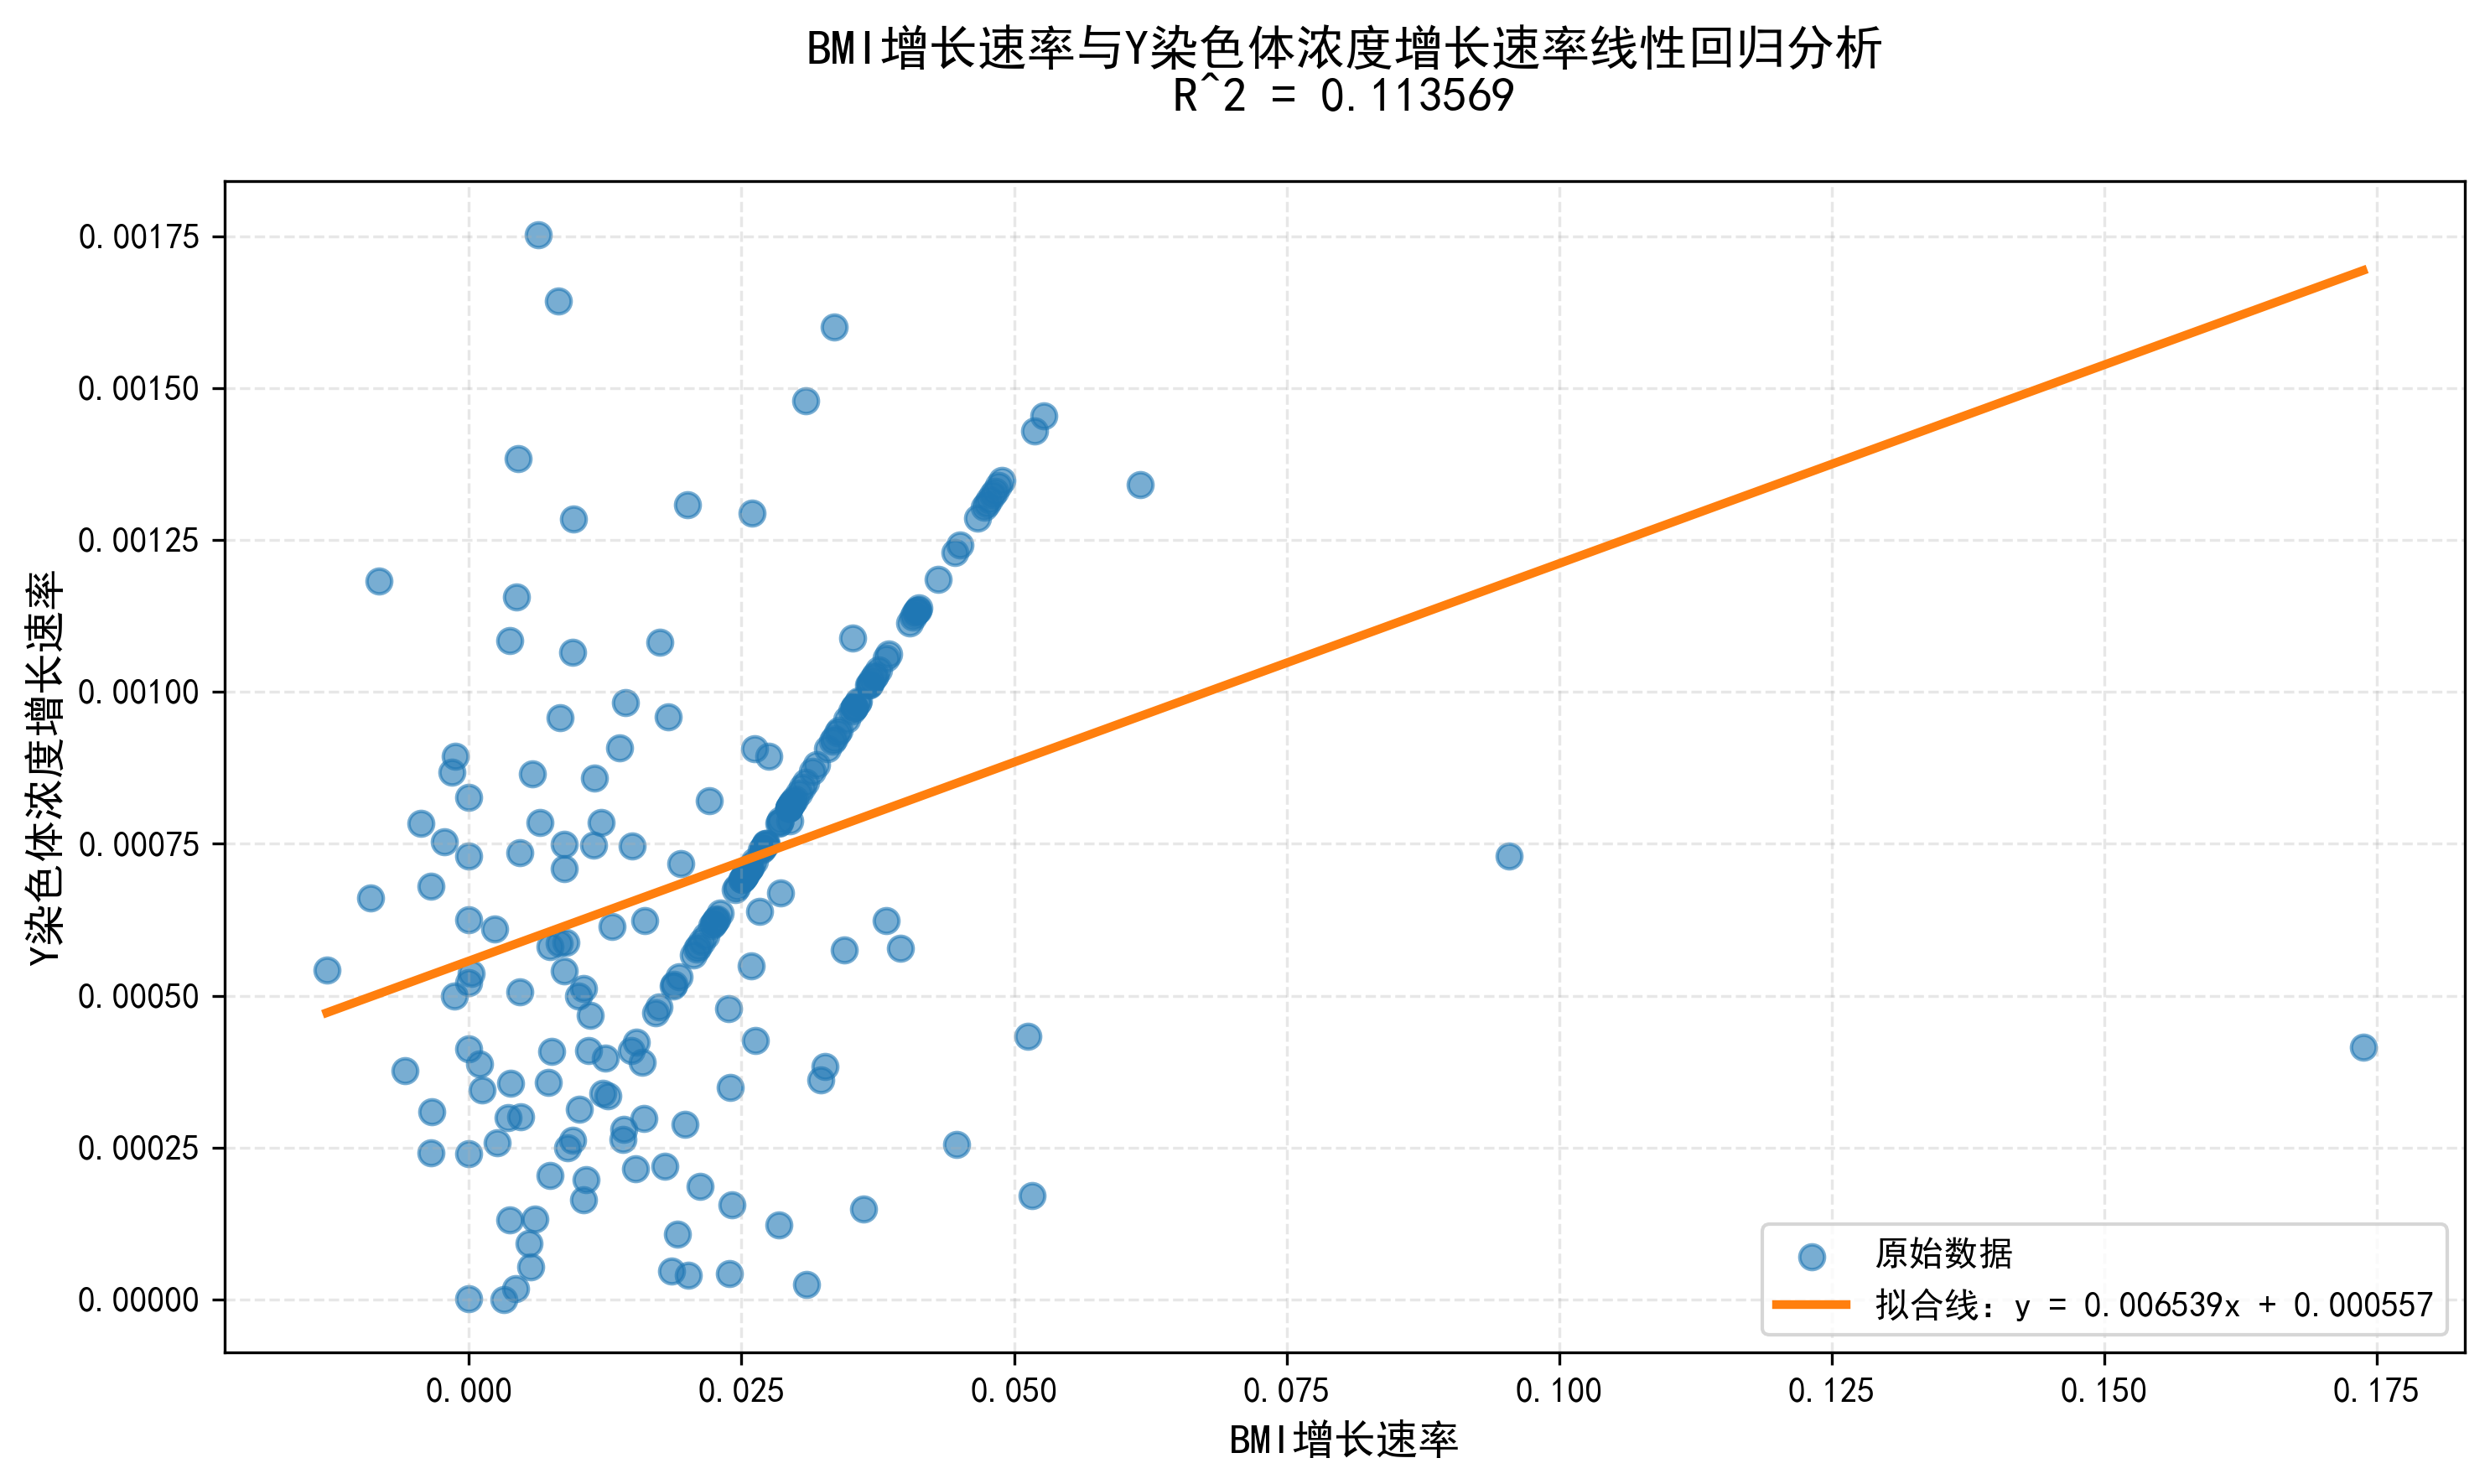
\includegraphics[width=\textwidth]{graph/linear_regression.png}
        \label{fig:sub2}
    \end{subfigure}
    \label{fig:two}  % 整体标签
\end{figure}

为探究BMI是否影响Y染色体浓度的增长速率,我们分析了每位孕妇的BMI增长率与Y染色体浓度增长率的相
关性。散点图与线性拟合显示$R^2$值较小,拟合效果不理想,因此需要考虑其他模型形式。

\subsection{\textbf{模型选择思路}}
首先,我们先对每个人线性回归,发现了绝大多数人y和时间关系与y和增长率和BMI增长率关系,以此我们
判定,所有曲线都遵循一个共同的、内在的生物学规律,但由于个体差异,曲线的高度和形状会各不相同。

\textbf{1.从生物学机理出发}:

题目背景与临床知识表明,胎儿游离DNA浓度(此处体现为Y染色体浓度)随孕周增加而增长。这是因为随着
胎儿发育,其细胞凋亡释放到母体血液中的DNA总量增加。这种增长通常不是线性的,在早期增长缓慢,中后
期可能加速,符合指数增长或逻辑增长的生物学规律。因此,我们优先考虑非线性模型来捕捉孕周与浓度的关系。

而对于BMI与Y染色体的浓度关系,较高的BMI可能意味着更多的血液量和脂肪组织,理论上会对胎儿游离DNA浓
度产生一定的“稀释”效应。因此,我们假设BMI对Y染色体浓度存在一个负向影响将这一项加入模型,符合我们的生理学直觉。

\textbf{2.从数据结构出发}:

本研究的核心特征在于数据结构:每个孕妇有多次重复测量记录,导致数据点之间存在明显的组内相关性。
若采用普通最小二乘回归,将严重违背模型独立性假设,导致参数估计偏差和标准误低估。

\subsection{\textbf{混合模型建立}}
由以上分析,以上几点共同决定了\textbf{混合效应模型}(Mixed-Effects Model) 是处理该数据最合
适的框架,引用这个模型能有效刻画个体间变异,分离组内与组间差异,从而为固定效应提供更稳健的估计。
我们分别建立了三种模型:线性混合模型,非线性混合模型,GAMM,具体数据如下

\begin{table}[htbp]
    \centering
    \setlength{\tabcolsep}{2pt}  % 保持窄列间距
    \small  % 保持小字体
    \caption{三种混合建模对比分析表}
    \renewcommand{\arraystretch}{1.5}  % 行间距放大1.5倍(可调整为1.2/1.8等)
    % 用tabularx,将4列均设为X型(自动伸缩+换行)
    \begin{tabularx}{\linewidth}{@{}X X X X@{}}  % @{}消除两侧多余间距
        \toprule
        特征指标          & 线性混合模型 (LMM)                         & 非线性混合模型 (NLME) - 指数形式            & 广义可加混合模型 (GAMM)                                    \\
        \midrule
        模型形式          & Y $\sim$ BMI + G\_days + (1|Subject) & Y $\sim$ a * exp(b * G\_days)    & Y $\sim$ s(BMI) + s(G\_days) + s(Subject, bs="re") \\
        模型复杂度/灵活性     & 低 (严格线性假设)                           & 中 (预设非线性形式)                      & 高 (数据驱动非线性形式)                                      \\
        固定效应 - BMI    & -0.001376 (p $\leq$ 0.01)            & -                                & 平滑项显著 (p = 0.00764)                                \\
        固定效应 - 孕周     & 0.0004466 (p $\leq$ 0.001)           & 0.0088 (p $\leq$ 0.001)          & 平滑项高度显著 (p $\leq$ 2e-16)                           \\
        随机效应 - 个体方差   & 0.0008285(Std.Dev: 0.02878)          & 0.0001279(Std.Dev: 0.01131) (仅a) & 包含在 s(Subject) 中 (高度显著, p < 2e-16)                 \\
        残差方差          & 0.0002930(Std.Dev: 0.01712)          & 0.0002807(Std.Dev: 0.01675)      & Scale est. = 0.00027726                            \\
        拟合优度 - AIC    & -5025.5 (REML)                       & -5026.912                        & REML = -2536.1 (与AIC/BIC不可直接比较)                    \\
        拟合优度 - R²/解释度 & -                                    & -                                & Adj. $R^2$ = 0.753, Deviance Explained = 81\%      \\
        核心优势          & 简单直观,解释性强                            & 捕捉指数增长趋势,生物学解释性好                 & 无需预设形式,自动捕捉复杂非线性关系,拟合优度最高                          \\
        主要局限          & 可能忽略重要非线性关系,拟合度相对较低                  & 函数形式预设可能带来偏差,未包含BMI              & 结果为平滑曲线,缺乏参数化解析表达式                                 \\
        \bottomrule
    \end{tabularx}
    \label{tab:model_comparison}
\end{table}
综合对比分析:

\subsubsection{\textbf{模型复杂度与拟合优度}}
LMM 最为简单,但将复杂关系强制线性化,可能导致拟合不足(从残差和AIC均可看出)。

NLME 通过引入指数形式,更好地捕捉了Y浓度随孕周的核心增长趋势,其AIC值略优于LMM,表明在考虑模
型复杂度后拟合更好。但它未包含BMI,是一个重大缺陷。

GAMM 灵活性最高,同时纳入了BMI和孕周的非线性效应,并获得了最高的解释方差(81\%)。这强烈表明
变量间存在用简单线性或单一非线性无法捕捉的复杂关系。

\subsubsection{\textbf{孕周效应}}
LMM和NLME都证实孕周是极显著的影响因子。

GAMM不仅证实了其极显著性(p $\leq$ 2e-16),还通过有效自由度(edf = 4.682 $\geq$ 1) 表明孕周与Y浓度的
关系是显著非线性的,从数据上支持了NLME选用指数函数的思路是正确的。

\subsubsection{\textbf{BMI效应}}

LMM检测到BMI有显著的线性负效应(p $\leq$ 0.01)。

GAMM的发现更为深入:它不仅确认了BMI效应的显著性(p = 0.00764),更重要的是其有效自由度
(edf = 5.416 $\geq\geq$ 1) 表明BMI与Y浓度的关系是强烈的非线性,这意味着简单的线性项(如LMM中所用)
可能不足以准确描述其影响,BMI的影响可能在高低区间有所不同。

此外我们分别绘制了这三者对于原散点图的拟合曲线并绘制了这三者的各自的优劣图,如下:
\begin{figure}[H]
    \centering
    % 子图1:宽度占页面的45%(左右留空)
    \begin{subfigure}[b]{0.45\textwidth}  % [b]表示底部对齐
        \centering
        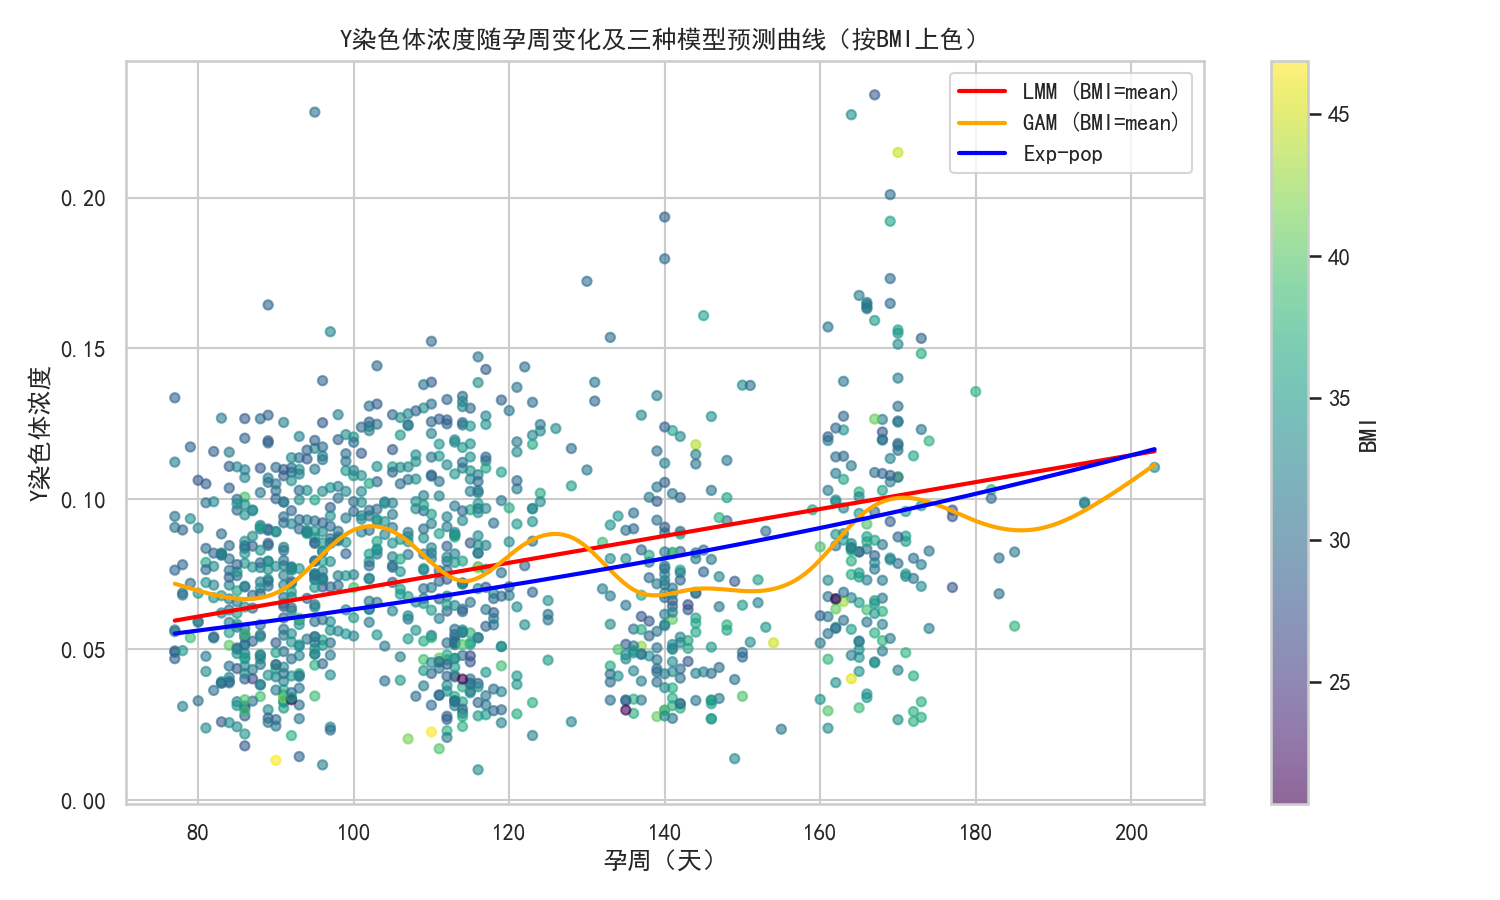
\includegraphics[width=\textwidth]{graph/y_vs_time_population_curves.png}  % 宽度=子图宽度
        \caption{拟合曲线}  % 子标题
        \label{fig:sub1}  % 子图标签
    \end{subfigure}
    \hspace{0.05\textwidth}  % 两图间距(5%页面宽度)
    % 子图2
    \begin{subfigure}[b]{0.45\textwidth}
        \centering
        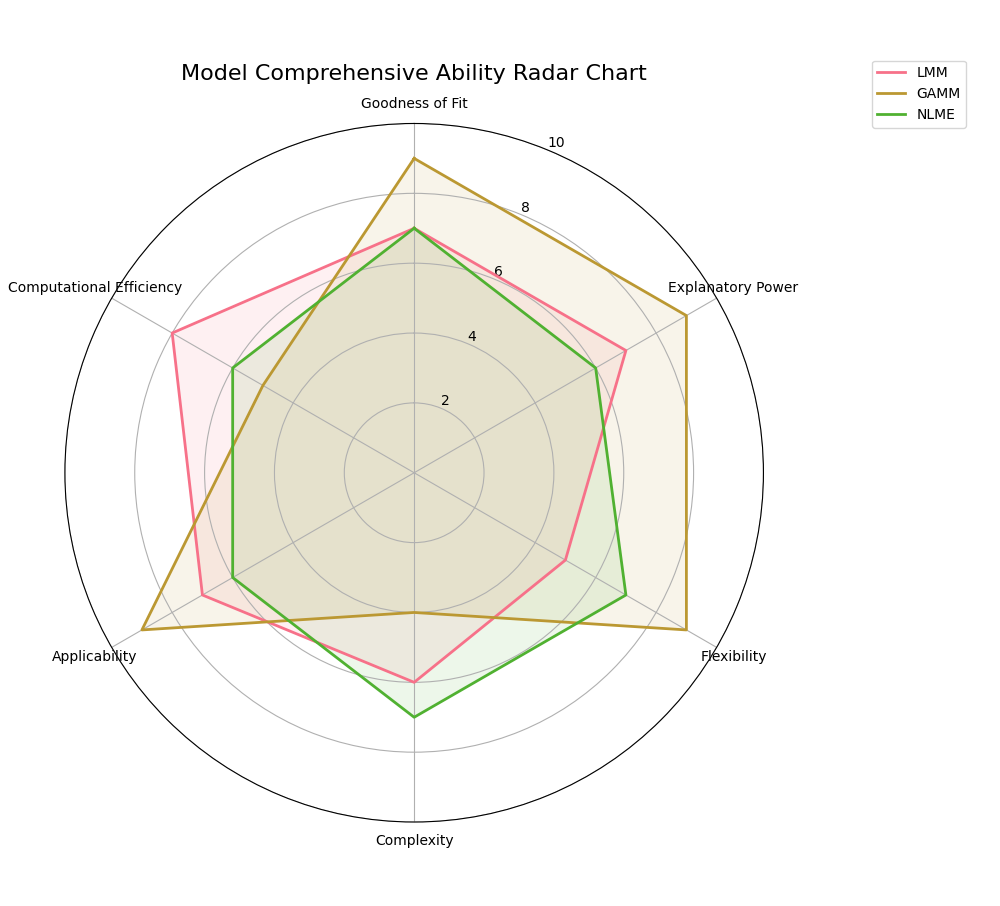
\includegraphics[width=\textwidth]{graph/ability.png}
        \caption{优势图}
        \label{fig:sub2}
    \end{subfigure}
    \label{fig:two}  % 整体标签
\end{figure}
总的来说,GAMM的拟合效果较好,我们选择GAMM方法进行建模。
\subsection{\textbf{GAMM模型的建立}}
为充分探索胎儿Y染色体浓度与孕妇孕周数和BMI之间可能存在的复杂非线性关系,避免预设模型形式的偏差,我们建立了广义可加混合模型(Generalized Additive Mixed Model, GAMM)。该模型不强制要求变量间满足特定的参数关系(如线性或指数关系),而是通过平滑函数灵活地拟合数据中潜在的非线性模式,同时通过随机效应项处理个体重复测量数据带来的相关性。

建立GAMM模型的具体形式如下:
\begin{gather}
    Y_{ij}=\beta_0+s_1(BMI_i)+s_2(G_{ij})+s_3(Subject_i)+\epsilon_{ij}\tag{3}
\end{gather}
其中:
\begin{itemize}
    \item $Y_{ij}$ 表示第 $i$ 个孕妇第 $j$ 次测量的Y染色体浓度
    \item $\beta_0$ 为模型截距项
    \item $s_1(BMI_i)$ 为BMI的平滑函数,用于捕捉BMI对Y染色体浓度的非线性影响
    \item $s_2(GestationalDays_{ij})$ 为孕周数的平滑函数,用于捕捉孕周对Y染色体浓度的非线性影响
    \item $s_3(Subject_i)$ 为针对孕妇个体的随机效应平滑项,用于捕捉个体特异性差异
    \item $\epsilon_{ij}$ 为残差项,假定服从正态分布:$\epsilon_{ij} \sim N(0, \sigma^2_\epsilon)$
\end{itemize}
模型采用薄板回归样条(Thin Plate Regression Splines)作为平滑函数的基础,使用REML
(Restricted Maximum Likelihood)方法进行参数估计,以保证方差分量估计的无偏性。
\subsection{\textbf{显著性检验}}
对建立的GAMM模型进行全面的显著性检验,结果如下:

\textbf{(1)平滑项显著性检验}

基于方差分析原理的显著性检验显示:

1.\textbf{BMI平滑项}($s_1(BMI_i)$):有效自由度(edf)= 5.416,参考自由度 = 6.263,F值 = 3.02,p值 = 0.00764**
\begin{itemize}
    \item 结果表明BMI对Y染色体浓度的影响具有高度显著的非线性特征(p $\leq$ 0.01)
    \item edf $\geq$ 1表明BMI与Y浓度间存在复杂的非线性关系,而非简单的线性关系
\end{itemize}

2.\textbf{孕周平滑项}($s_2(GestationalDays_{ij})$):有效自由度(edf)= 4.682,参考自由度 = 5.711,F值 = 77.86,p值 $\leq$ 2e-16***
\begin{itemize}
    \item 结果表明孕周对Y染色体浓度的影响极显著(p $\leq$ 0.001)
    \item edf = 4.682 $\geq$ 1证实了孕周与Y浓度间存在显著的非线性关系
\end{itemize}

3.\textbf{个体随机效应项}($s_3(Subject_i)$):有效自由度(edf)= 240.736,参考自由度 = 266.000,F值 = 10.58,p值 $\leq$ 2e-16***
\begin{itemize}
    \item 结果表明不同孕妇个体间存在极显著的差异性(p $\leq$ 0.001)
    \item 证明使用混合效应模型处理重复测量数据的必要性
\end{itemize}

\textbf{(2)模型拟合优度检验}
\begin{itemize}
    \item 调整后$R^2$ = 0.753,表明模型能够解释Y染色体浓度75.3\%的变异
    \item 偏差解释率 = 81\%,表明模型对数据偏差的解释程度较高
    \item 尺度参数估计值 = 0.00027726,反映了模型的残差方差
    \item REML准则值 = -2536.1,用于模型比较(数值越小表示拟合越好)
\end{itemize}

GAMM模型的结果为后续参数化模型(非线性混合效应模型)的选择提供了坚实的数据驱动依据,证实了孕
周和BMI与Y染色体浓度间均存在显著的非线性关系。
%%%%%%%%%%%%%%%%%%%%%%%%%%%%%%%%%%%%%%%%%%%%%%%%%%%%%%%%%%%%%%%%%%%%%%%%%%%%%%%%%%%%
%%%%%%%%%%%%%%%%%%%%%%%%%%%%%%%%%%%%%%%%%%%%%%%%%%%%%%%%%%%%%%%%%%%%%%%%%%%%%%%%%%%%
%                                   QUESTION TWO                                   %
%%%%%%%%%%%%%%%%%%%%%%%%%%%%%%%%%%%%%%%%%%%%%%%%%%%%%%%%%%%%%%%%%%%%%%%%%%%%%%%%%%%%
%%%%%%%%%%%%%%%%%%%%%%%%%%%%%%%%%%%%%%%%%%%%%%%%%%%%%%%%%%%%%%%%%%%%%%%%%%%%%%%%%%%%
\section{\textbf{问题二模型建立求解}}
\subsection{\textbf{数据预处理}}
本问题旨在探究孕妇BMI对胎儿Y染色体浓度最早达标时间的影响。考虑到同一孕妇的BMI随时间变化幅度较小
(个体内变异),且个体间差异远大于时间变化量,为提高分析的准确性和可靠性,我们采用每位孕妇多次BMI
测量的平均值作为其代表值进行后续统计分析。

为合理区分样本并便于计算NIPT最佳时点,我们依据Y染色体浓度达标情况对孕妇进行了科学分组:
\begin{itemize}
    \item 第一组\textbf{(始终达标组)}:从首次检测开始Y染色体浓度即达到或超过4\%的样本。该组数据保存在 `bmi\_Y\_always\_can\_test\_result.xlsx`中,包含孕妇代码、平均BMI和最早达标天数(即首次检测时间)。
    \item 第二组\textbf{(中间达标组)}:初始检测未达标但后续检测达标的样本。该组数据保存在 \\
          `bmi\_Y\_middle\_result.xlsx`中,包含孕妇代码、平均BMI和预测达标天数(通过\textbf{插值法}计算获得,详见附录代码Line XX)。
    \item 第三组\textbf{(从不达标组)}:所有检测中Y染色体浓度均未达标的样本。该组数据保存在 \\
          `bmi\_Y\_cannot\_test\_result.xlsx`中,包含孕妇代码、平均BMI和最晚达标天数(即末次检测时间)。
\end{itemize}

为确保数据质量,若某样本曾达标但后续检测又低于4\%,则视为无效样本并予以剔除。经上述处理,最终获得
有效样本总量为230例。其中,第一组186例(占比80.87\%),第二组37例(占比16.09\%),第三组7例(占
比3.04\%)。这一分组策略确保了后续分析的可靠性和代表性。

\subsection{\textbf{BMI划分与聚类分析}}
为探究BMI对Y染色体浓度达标时间的影响模式,我们采用聚类算法对孕妇平均BMI进行科学细分。首先,通过肘
部法则确定最佳聚类数量(图1)。结果显示,当聚类数超过5时,距离平方和下降速率显著降低,故选择聚类
数k=5作为最优解。
% 单个图片
\begin{figure}[H]  % [H]表示强制当前位置(可选参数:h=此处,t=顶部,b=底部,p=单独页)
    \centering  % 图片居中
    % 插入图片:width=0.8\textwidth 表示占页面宽度的80%(可调整)
    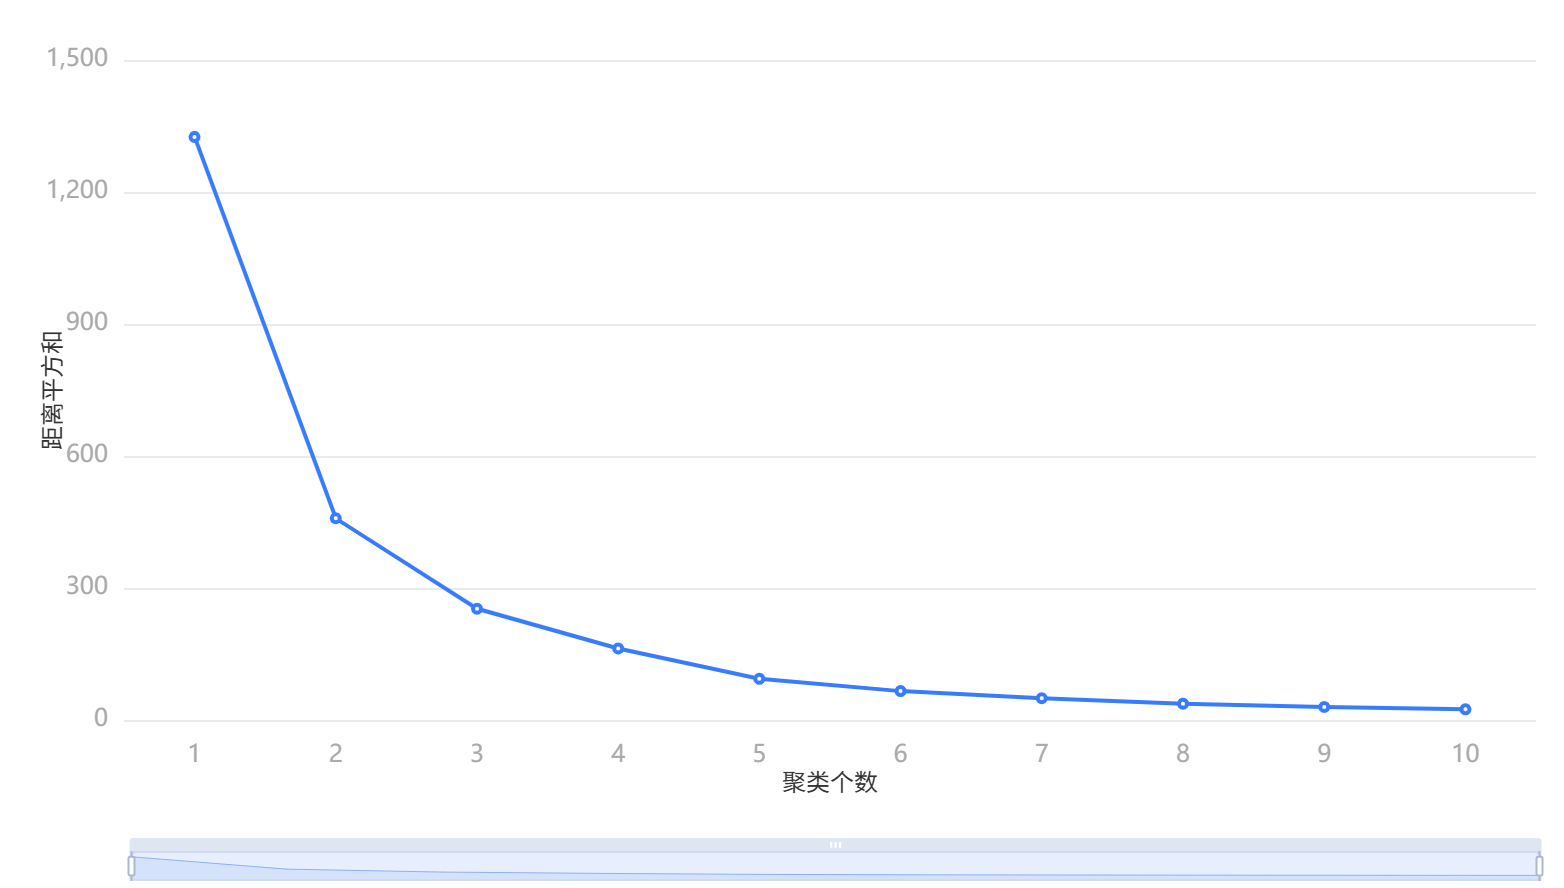
\includegraphics[width=0.8\textwidth]{graph/zhoubu.png}  % 替换为实际图片路径
    \caption{肘部法则图}  % 图片标题
    \label{fig:single}  % 标签(用于交叉引用:\ref{fig:single})
\end{figure}

基于此,我们对孕妇平均BMI与Y染色体浓度进行了K-means聚类分析,结果如图2所示。聚类结果清晰地展示
了不同BMI区间与Y染色体浓度的关联模式。
% 单个图片
\begin{figure}[H]  % [H]表示强制当前位置(可选参数:h=此处,t=顶部,b=底部,p=单独页)
    \centering  % 图片居中
    % 插入图片:width=0.8\textwidth 表示占页面宽度的80%(可调整)
    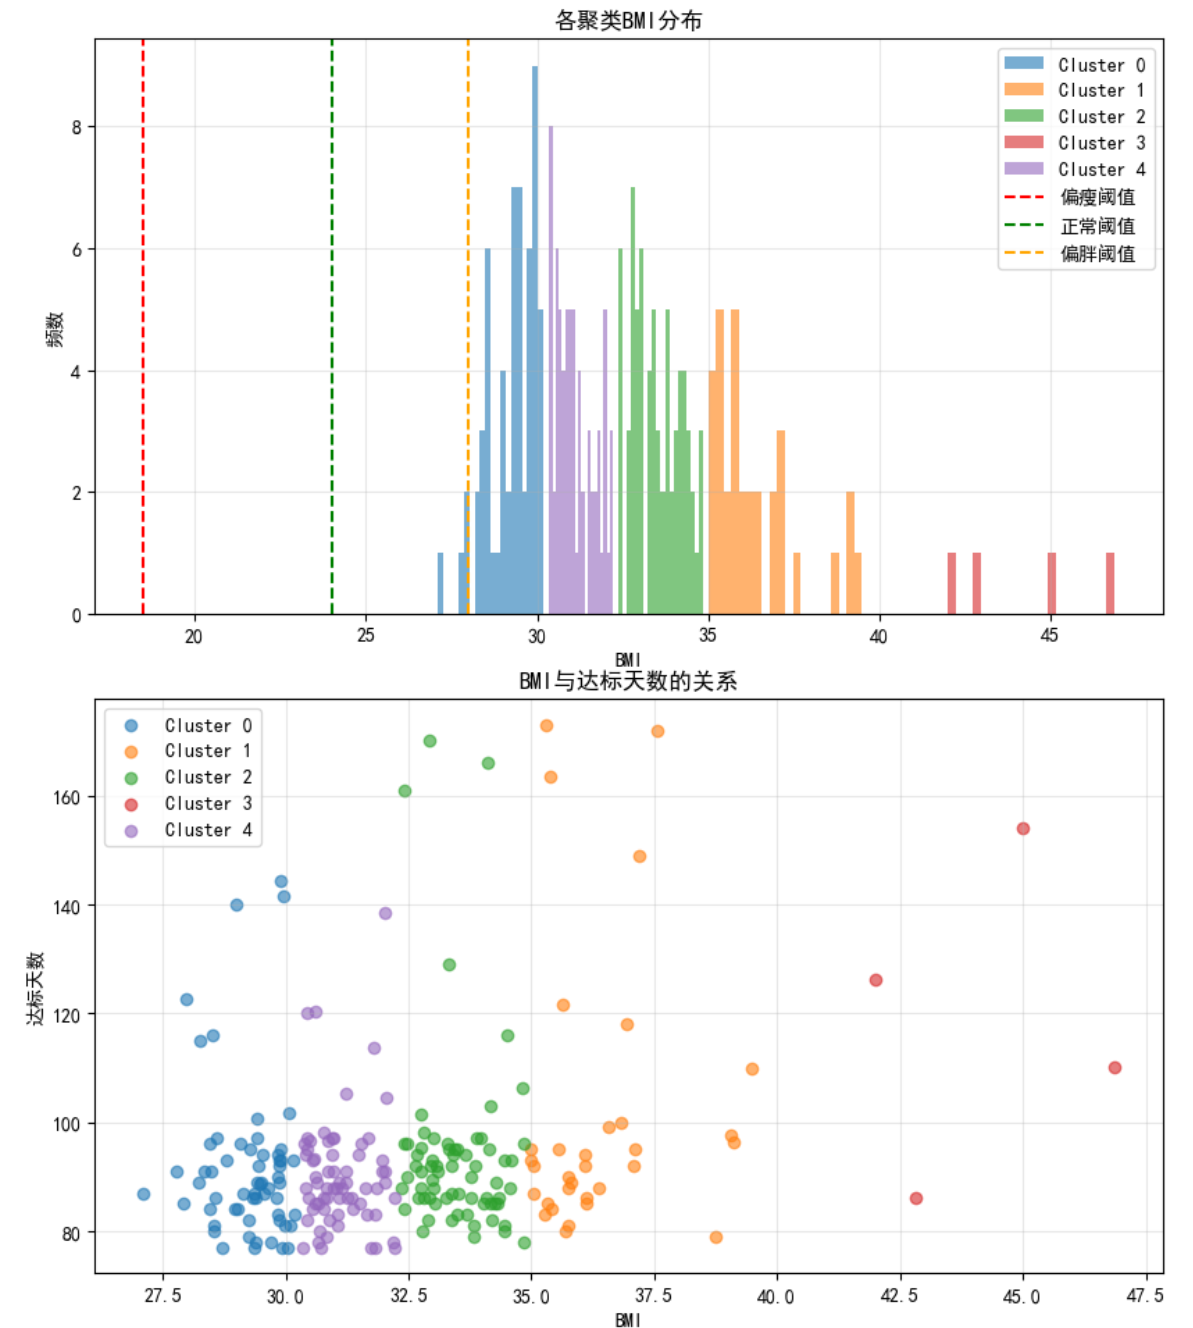
\includegraphics[width=0.8\textwidth]{graph/julei1.png}  % 替换为实际图片路径
    \caption{聚类结果散点图}  % 图片标题
    \label{fig:single}  % 标签(用于交叉引用:\ref{fig:single})
\end{figure}

\subsection{\textbf{聚类分类评价}}
为进一步评估聚类质量,我们计算了三个内部评价指标:
\begin{itemize}
    \item \textbf{轮廓系数}:0.551(轮廓系数取值范围[-1,1],值越大表示同类样本越相近,不同类样本越远离,一般不可能大于0.7 )
          \begin{gather}
              s(i)=\frac{b(i)-a(i)}{\max{a(i),b(i)}} \tag{5}
          \end{gather}
          \( a(i) \): 样本 \( i \) 到\textbf{同一簇内}所有其他样本的平均距离。\textbf{(凝聚度)}
          \textbf{\( b(i) \)}: 样本 \( i \) 到\textbf{其他某个簇}的所有样本的平均距离。计算样本 \( i \)
          与所有\textbf{非本身所在簇}的的平均距离,然后取其中的\textbf{最小值}。\textbf{(分离度)}

    \item \textbf{DBI指数}:0.517(值越小表示类内紧密度越高,类间分离度越好,<0.7可接受 )
          \begin{gather}
              DBI = \frac{1}{K} \sum_{i=1}^{K} \max_{j \neq i} R_{ij} \tag{6}
          \end{gather}
          K: 簇的个数。$R_{ij}$: 簇 $i$ 和簇 $j$ 之间的\textbf{相似度}$s_i$: 簇 $i$ 的簇内散度,即簇内所有样本到其质心$c_i$的平均距离。
          $d_{ij}$: 簇 $i$ 的质心$ c_i$ 与簇$j$ 的质心 $c_j$ 之间的距离(通常使用欧氏距离)。

    \item \textbf{CH指数}:701.814(值越大表示聚类效果越优 )
          \begin{gather}
              CH = \frac{\text{SS}_B / (K - 1)}{\text{SS}_W / (N - K)} \tag{7}
          \end{gather}
          N: 数据集中的总样本数。K: 簇的个数。$\text{SS}_B$: \textbf{簇间离散度}(Between-Cluster Sum
          of Squares)。所有簇的质心 $c_k$ 与全局质心 $c$ 的距离平方和,并按簇大小加权。
          $\text{SS}_W$: \textbf{簇内离散度}(Within-Cluster Sum of Squares)。所有样本点到其所属簇的质心的距离平方和。

          \subsection{\textbf{NIPT时点计算}}

\end{itemize}
上述指标综合表明,本次聚类效果良好,各类别内部样本相似度高,类别之间差异明显,分类结果可靠有效,为后续分析奠定了坚实基础。
\subsection{\textbf{NIPT时点计算}}
\subsubsection{\textbf{方法原理与模型构建}}
为确定各BMI分组的最佳NIPT检测时点,本研究构建了一个基于风险-效用权衡的优化模型。该模型综合考虑了早期检测与晚期检测的双重风险,通过数学优化方法寻找使总体风险最小化的检测时间点。

\textbf{风险函数定义:}
\begin{itemize}
    \item 早期检测风险$(R_{early})$:检测时间过早可能导致Y染色体浓度尚未达标,造成假阴性结果。我们采用指数衰减函数模拟这一风险:
          \[
              R_{\text{early}}(t) = 2.0 \cdot e^{-t/50} \tag{1}
          \]
          该函数从初始值2.0开始,随孕期增加呈指数衰减,反映早期预测的高风险性。
    \item 晚期检测风险$(R_{late})$:检测时间过晚则可能错过最佳干预时机。我们采用分段函数描述这一风险:
          \[
              R_{\text{late}}(t) =
              \begin{cases}
                  0.1                                                  & t < 84             \\
                  0.1 + 0.9 \cdot \left( \frac{t-84}{189-84} \right)^2 & 84 \leq t \leq 189 \\
                  1.0                                                  & t > 189
              \end{cases} \tag{2}
          \]
          该函数在84天前保持低风险(0.1),84-189天间以二次函数形式增长,189天后达到最高风险(1.0)。
\end{itemize}
\textbf{效用函数构建:}

基于累积达标概率F(t)(通过Kaplan-Meier估计器计算)和上述风险函数,我们构建综合效用函数:
\[
    U(t) = (1 - F(t)) \cdot R_{\text{early}}(t) + F(t) \cdot R_{\text{late}}(t)\\
\]
其中F(t)表示在时间t之前Y染色体浓度达到4\%的累积概率。

\textbf{优化目标:}

通过最小化效用函数U(t)确定最佳检测时点:
\[
    t^* = \arg\min_{t \in [0, T_{\text{max}}]} U(t) \\
\]
其中$T_{max}$为观察期上限。

\subsubsection{\textbf{计算流程与实施}}
本研究采用以下步骤计算各BMI分组的最佳NIPT时点:

1. \textbf{数据准备与分组}:基于聚类分析得到的5个BMI区间,将样本分为相应组别。

2. \textbf{生存分析}:对每个BMI分组,应用Kaplan-Meier方法估计累积达标函数$F(t)$,处理右删失数据(始终达标组和从不达标组)。

3. \textbf{效用函数计算}:在时间域$[0, T_{max}]$上离散采样,计算各时间点的效用值$U(t)$。

4. \textbf{优化求解}:采用有界优化算法(Bounded方法)寻找使$U(t)$最小化的时间点t*。

5. \textbf{误差分析}:通过蒙特卡洛模拟(100次重复)评估检测误差对最优时点稳定性的影响。
\subsubsection{结果与分析}
表2展示了各BMI分组的最佳NIPT时点及相应指标:
\begin{table}[htbp]
    \centering
    \caption{各BMI分组最佳NIPT时点计算结果}
    \begin{tabular*}{\linewidth}{@{\extracolsep{\fill}}c c c c c}
        \toprule  % 顶部粗线
        BMI分组 & 最优时点(天) & 最小效用值 & 风险水平 & 样本量 \\
        \midrule  % 表头与内容间的细线
        $\leq$30.26 & 89.5 & 0.1299 & 7.696559&59 \\
        30.26-32.30&90.8&0.1360&7.3511&68 \\
        32.30-34.92&90.8&0.1359&7.3591&69\\
        34.92-39.49&99.4&0.1569&6.3753&33\\
        $\geq$39.49&110.7&0.1884&5.3090&4\\
        \bottomrule  % 底部粗线
    \end{tabular*}
    \label{tab:crops_booktabs}
\end{table}
结果表明,随着BMI增加,最佳检测时点相应延后,而效用值逐渐增加(风险水平降低)。这一趋势与临床观察
一致,高BMI孕妇需要更长时间等待Y染色体浓度达标,但一旦达标,其检测风险相对较低。

图3展示了其中一组的典型分析结果,包括累积达标曲线、效用函数曲线及最优时点标注。(剩余的会在附录中给出)
% 单个图片
\begin{figure}[H]  % [H]表示强制当前位置(可选参数:h=此处,t=顶部,b=底部,p=单独页)
    \centering  % 图片居中
    % 插入图片:width=0.8\textwidth 表示占页面宽度的80%(可调整)
    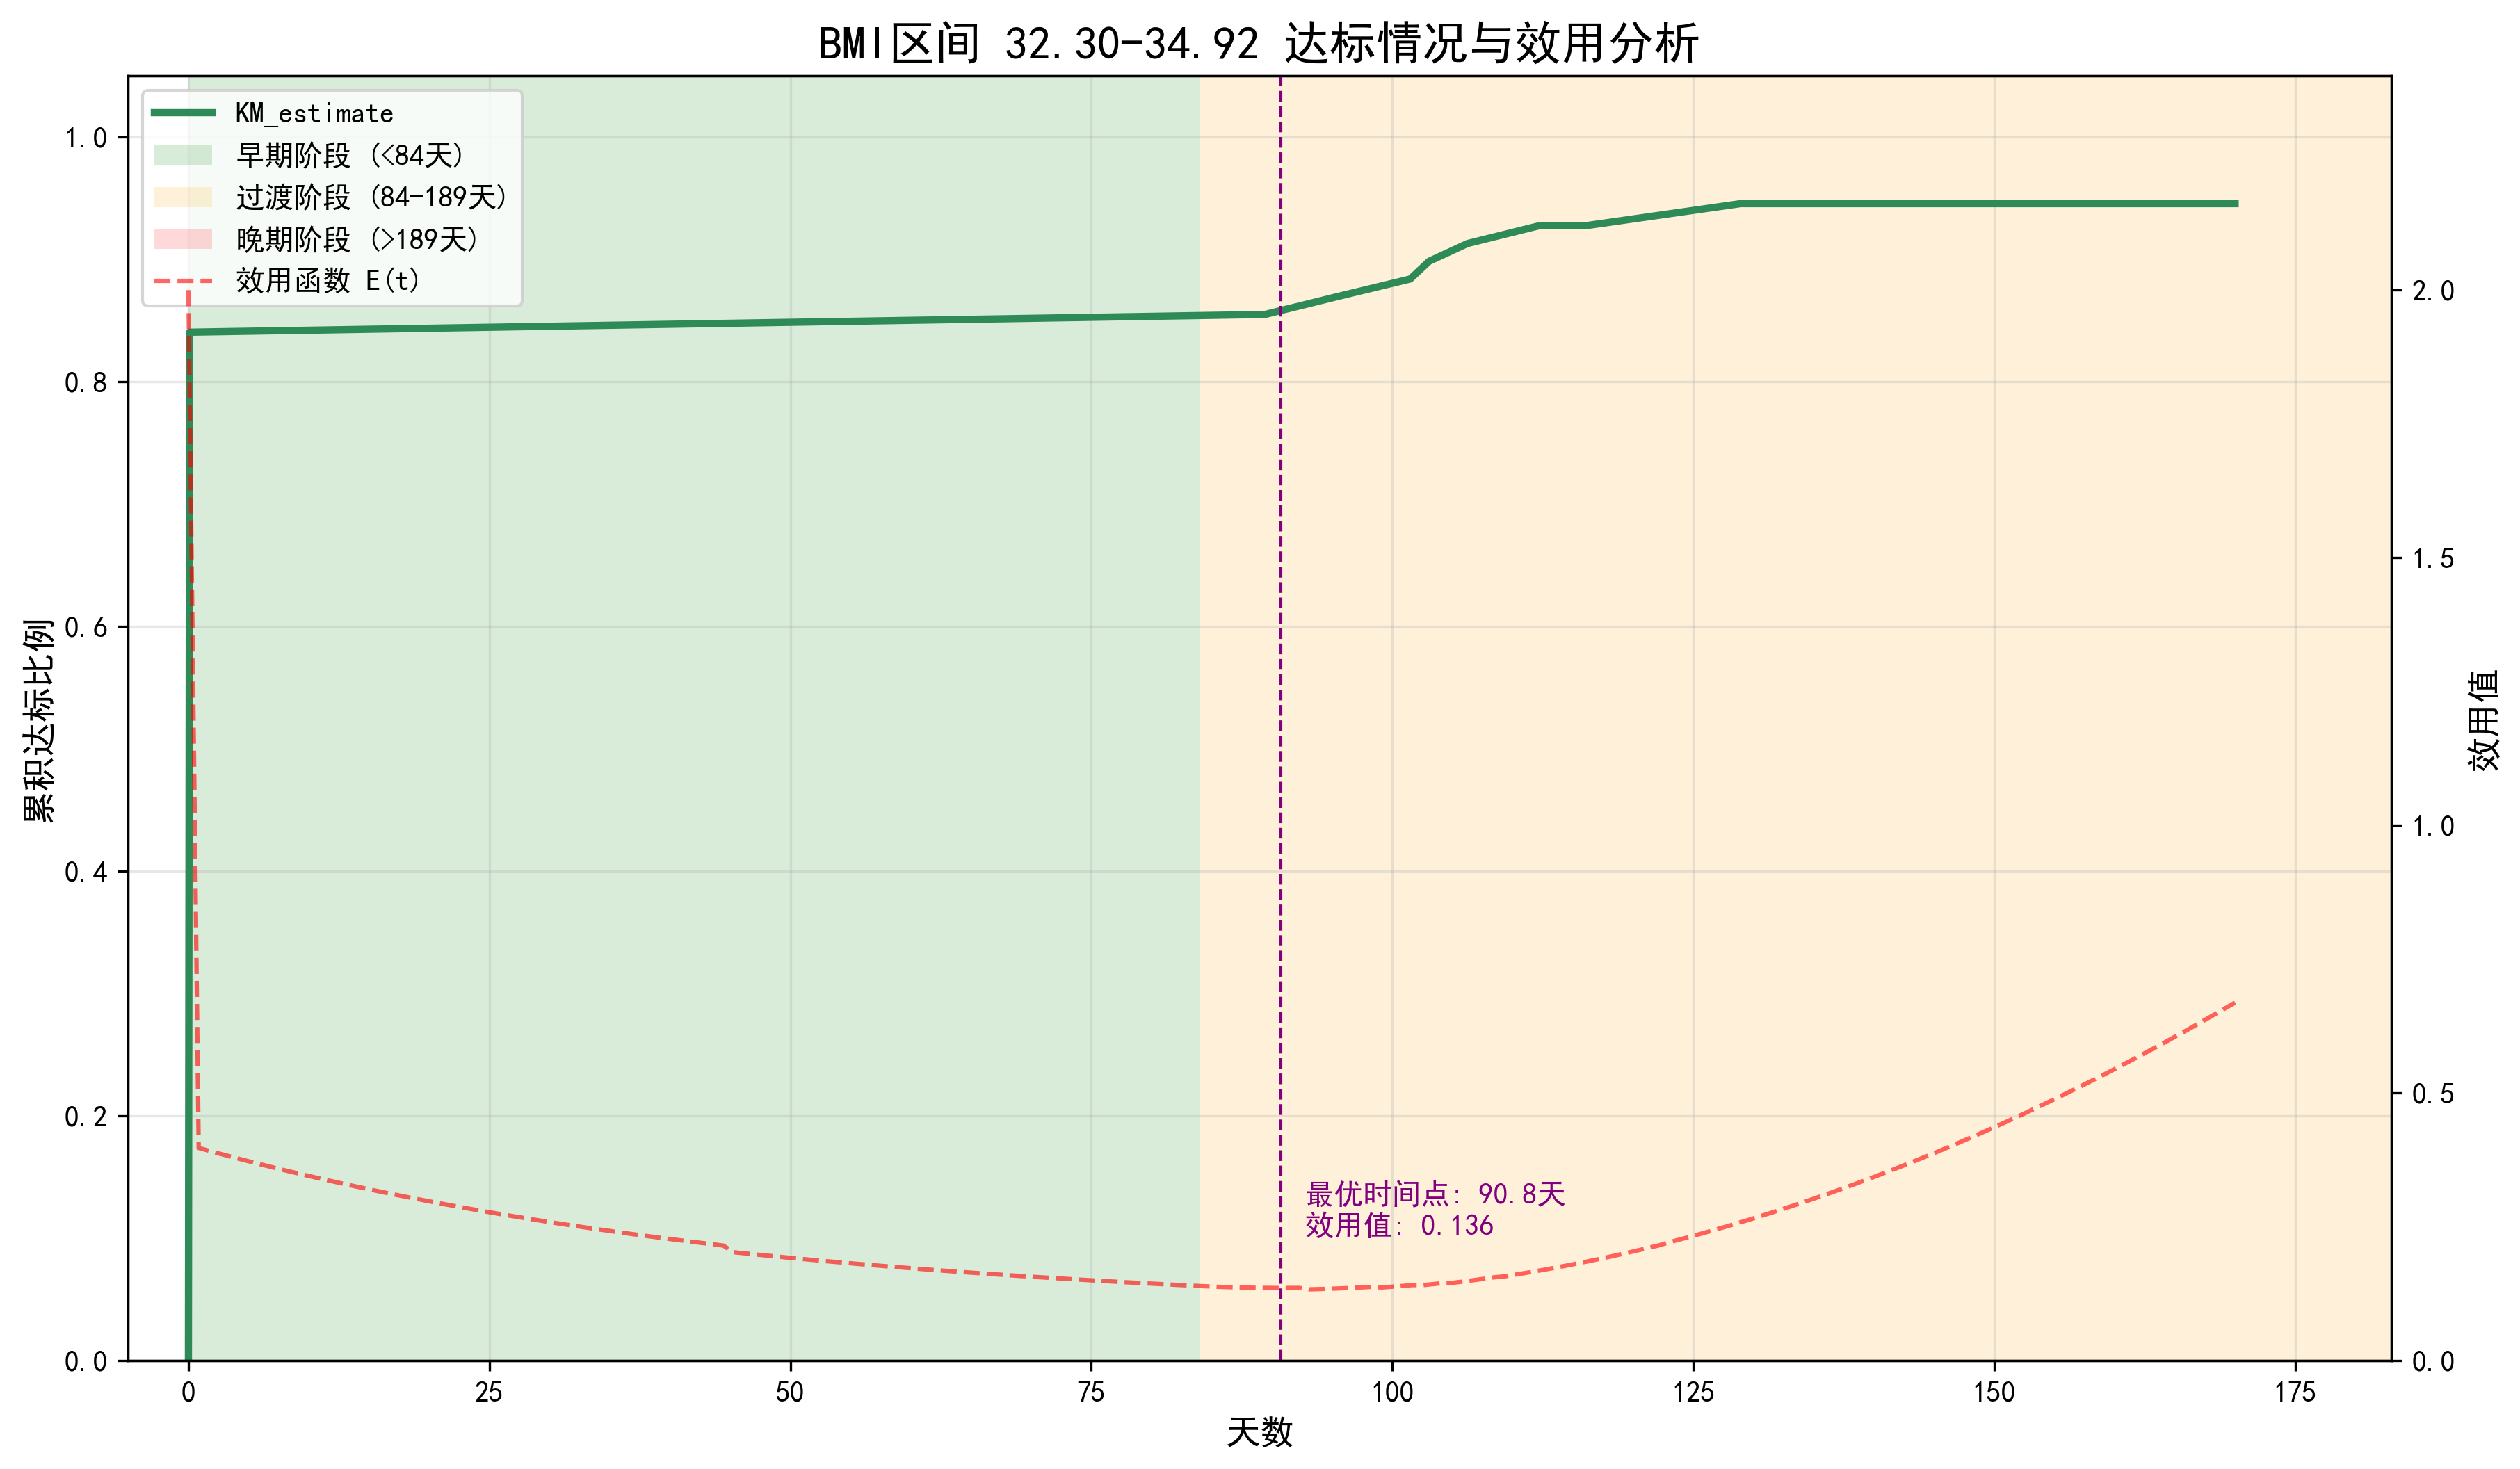
\includegraphics[width=0.8\textwidth]{graph/BMI_32.30_34.92_utility_analysis.png}  % 替换为实际图片路径
    \caption{32.30-34.92组}  % 图片标题
    \label{fig:single}  % 标签(用于交叉引用:\ref{fig:single})
\end{figure}
\subsubsection{\textbf{误差敏感性分析}}
为评估检测误差对结果稳定性的影响,我们进行了蒙特卡洛模拟分析。假设检测误差服从正态分布(标准差=
5\%),对每个BMI分组进行100次重复模拟。

表3a和表3b展示了误差分析结果:
\begin{table}[htbp]
    \centering
    \caption{\textbf{表3a:检测误差对最优时点的影响分析(时点相关指标)}}
    \begin{tabular*}{\linewidth}{@{\extracolsep{\fill}}c c c c c}
        \toprule  % 顶部粗线
        BMI分组 & 原始最优时点(天) & 模拟最优时点均值(天)&时点标准差(天)& 95\%置信区间(天)\\
        \midrule  % 表头与内容间的细线
        <30.26 & 89.51&90.05 & 1.56 & (89.74, 90.35)\\
        30.26-32.30 & 90.79 & 92.64 & 2.52 & (92.14, 93.13)\\
        32.30-34.92 & 90.76 & 91.19 & 1.39 & (90.92, 91.46)\\
        34.92-39.49 & 99.44 & 100.04 & 2.37 & (99.58, 100.51)\\
        >39.49 & 110.75 & 110.11 & 3.49 & (109.43, 110.79)\\
        \bottomrule  % 底部粗线
    \end{tabular*}
    \label{tab:crops_booktabs}
\end{table}
\begin{table}[htbp]
    \centering
    \setlength{\tabcolsep}{2pt}  % 列间距从6pt缩到2pt(可调整)
    \small  % 字体缩小一级(可选:\footnotesize 更小)
    \caption{\textbf{表3b:检测误差对最优时点的影响分析(效用值与风险水平相关指标)}}
    \begin{tabular*}{\linewidth}{@{\extracolsep{\fill}}c c c c c c c}
        \toprule  % 顶部粗线
        BMI分组&原始最小效用值&模拟最小效用值均值&效用值标准差&原始风险水平&模拟风险水平均值&风险水平标准差\\
        \midrule  % 表头与内容间的细线
        $\leq$30.26&0.1299&0.1274&0.0023&7.6965&7.8546&0.1448\\
        30.26-32.30&0.1360&0.1322&0.0032&7.3511&7.5677&0.1808\\
        32.30-34.92&0.1359&0.1336&0.0021&7.3591&7.4851&0.1199\\
        34.92-39.49&0.1569&0.1594&0.0027&6.3753&6.2773&0.1072\\
        $\geq$39.49&0.1884&0.1829&0.0124&5.3090&5.4973&0.4362\\
        \bottomrule  % 底部粗线
    \end{tabular*}
    \label{tab:crops_booktabs}
\end{table}
结果表明:

1. 检测误差对最优时点的影响较小(时点变异系数<3.5\%),模型具有较好的稳健性。

2. 高BMI分组对检测误差更为敏感,时点波动范围更大。

3. 所有分组的95\%置信区间范围合理,验证了推荐时点的可靠性。

4. 效用值和风险水平的变异程度相对较小,表明模型对这些指标的预测较为稳定。

图4展示了其中一组的误差模拟的详细结果,包括时点分布、效用值分布及风险分布。(其余的会在附录中给出)

\begin{figure}[H]  % [H]表示强制当前位置(可选参数:h=此处,t=顶部,b=底部,p=单独页)
    \centering  % 图片居中
    % 插入图片:width=0.8\textwidth 表示占页面宽度的80%(可调整)
    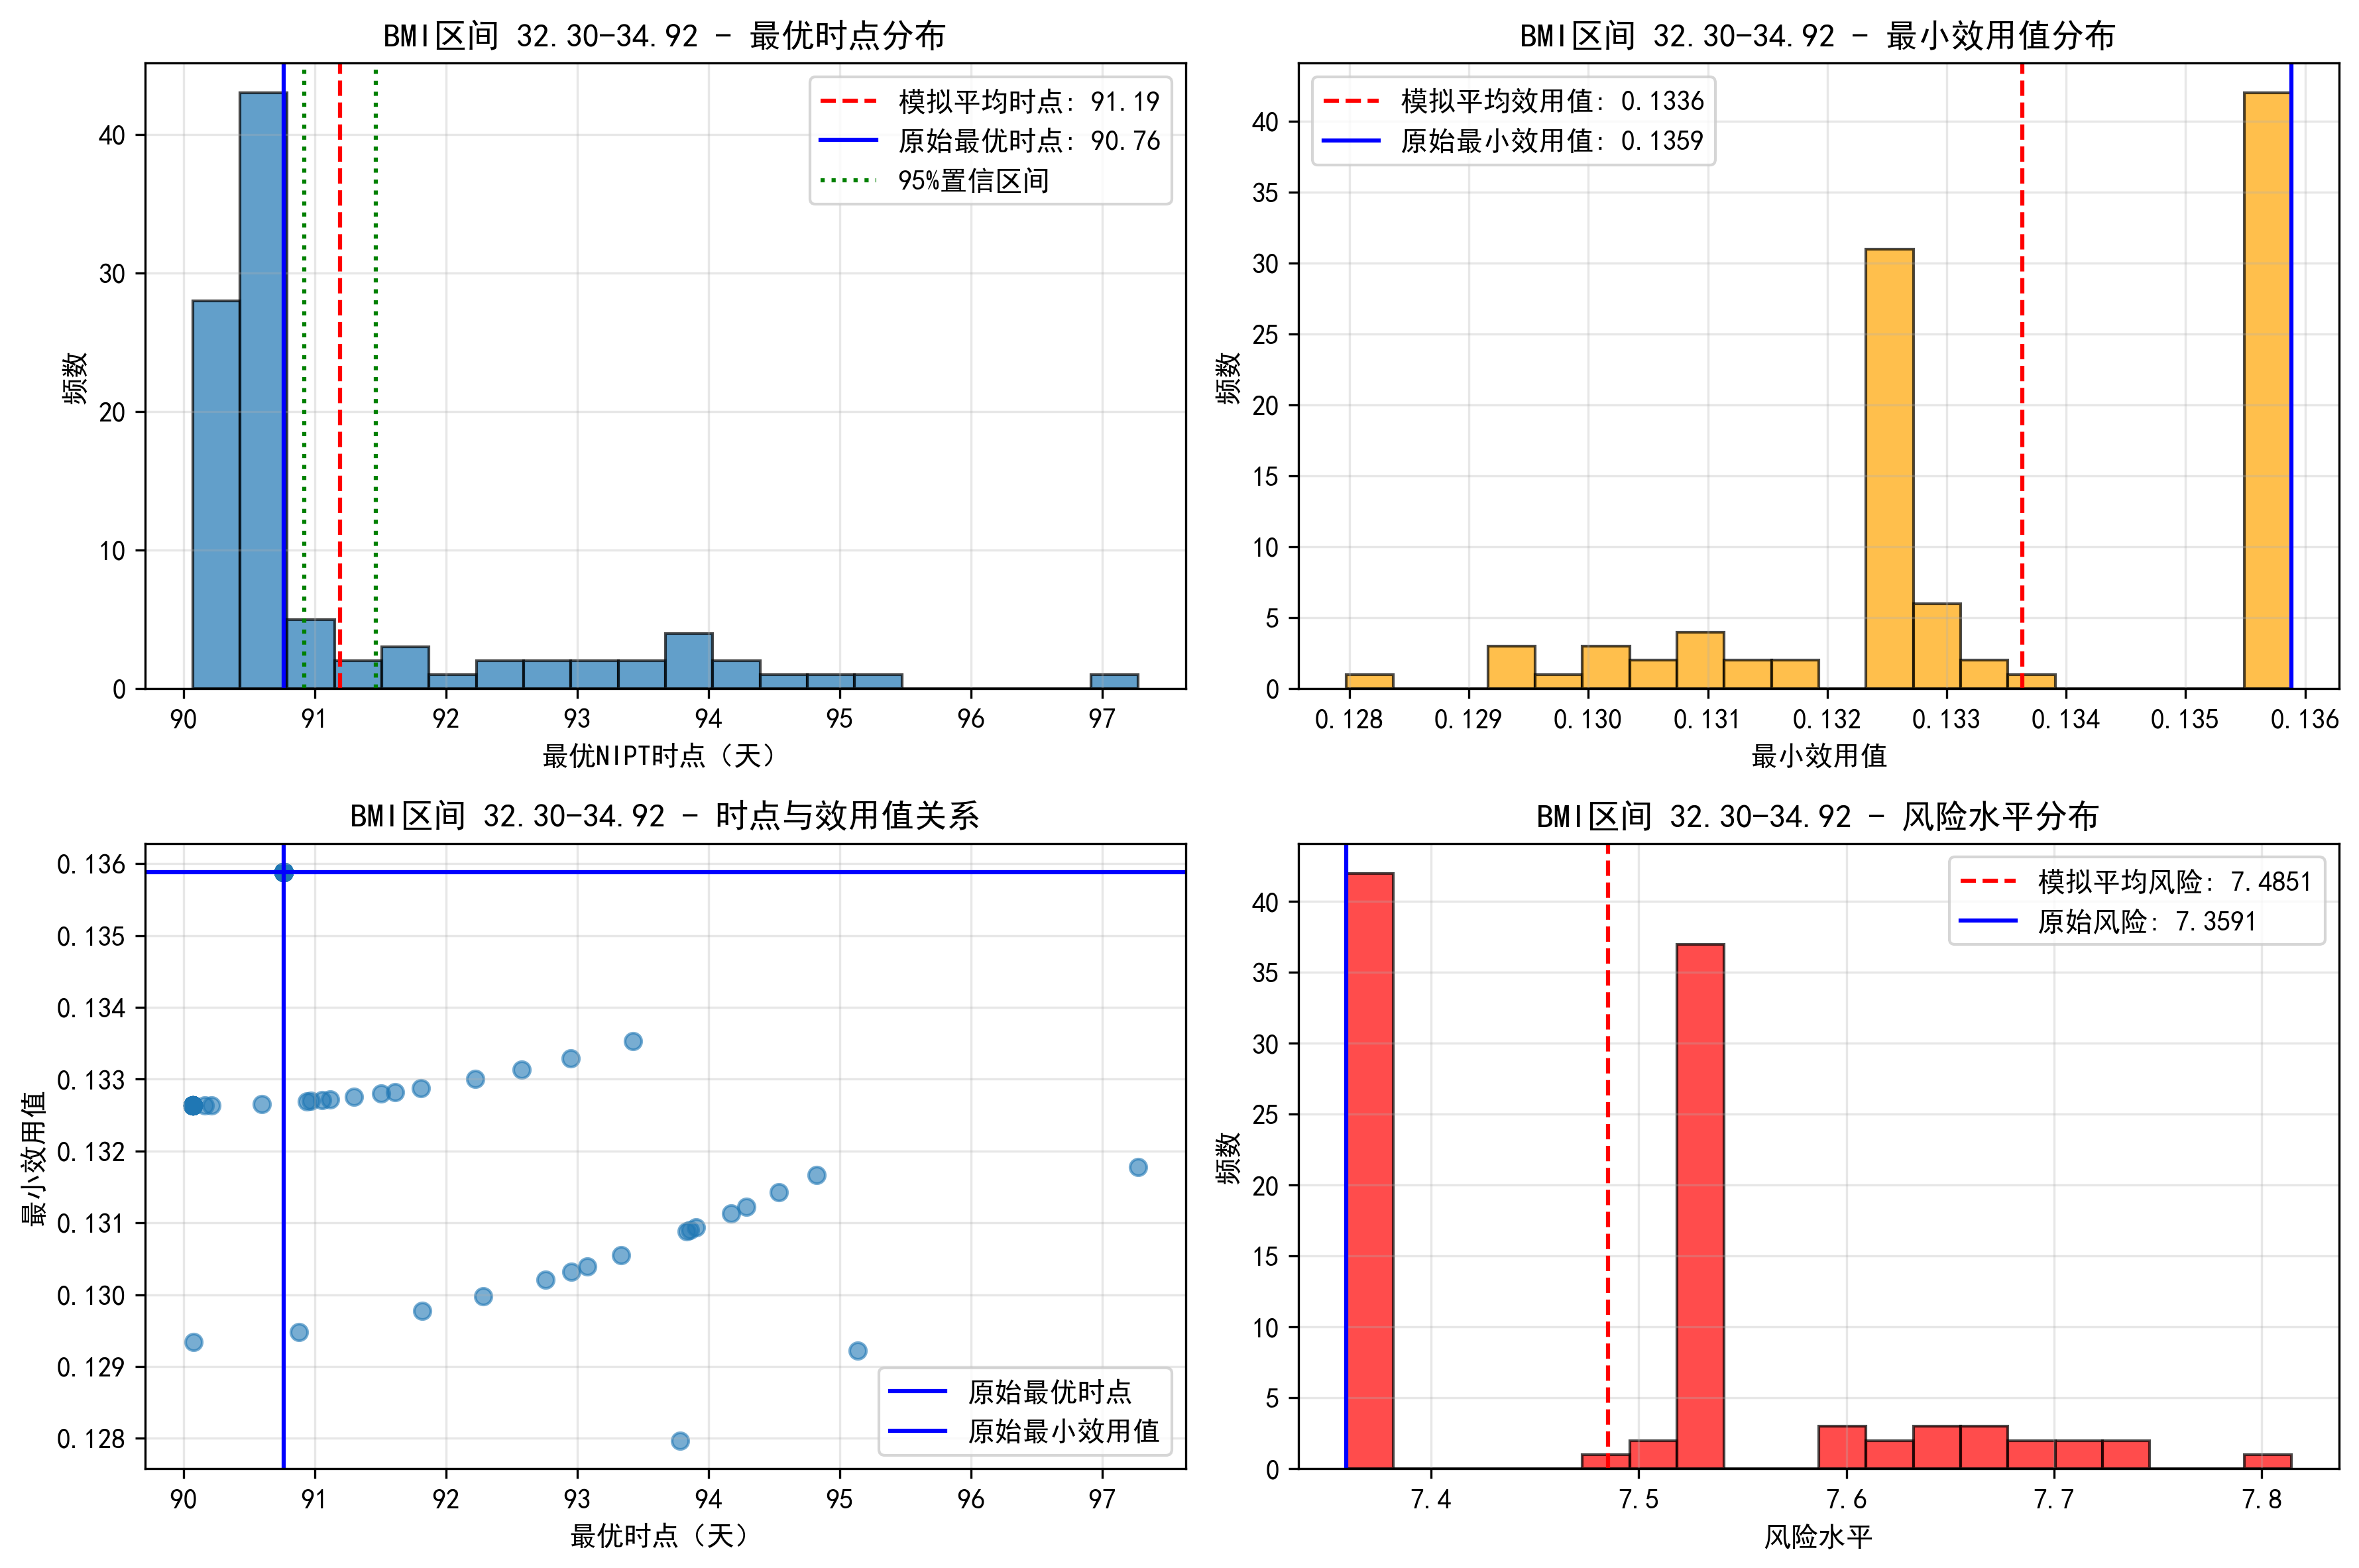
\includegraphics[width=0.8\textwidth]{graph/error_analysis_BMI_32.30-34.92.png}  % 替换为实际图片路径
    \caption{32.30-34.92组}  % 图片标题
    \label{fig:single}  % 标签(用于交叉引用:\ref{fig:single})
\end{figure}

\subsubsection{\textbf{创新与亮点}}
本研究在NIPT时点计算方面具有以下创新点:

1. \textbf{综合风险建模}:首次将早期检测风险与晚期检测风险同时纳入考量,构建了更符合临床实际的效用函数。

2. \textbf{生存分析方法应用}:采用Kaplan-Meier方法处理右删失数据,提高了累积达标概率估计的准确性。

3. \textbf{蒙特卡洛误差分析}:通过模拟检测误差的影响,量化了模型的稳健性,为临床决策提供了可靠性评估。

4. \textbf{BMI分层优化}:针对不同BMI群体分别计算最优时点,实现了个性化检测推荐。

本研究提供的NIPT时点推荐方案,不仅考虑了检测准确性,还综合评估了时间相关的风险因素,为临床实践提
供了科学依据。结果表明,基于BMI分层的个性化检测时点选择,能够有效降低孕妇的潜在风险,提高检测效率。
%%%%%%%%%%%%%%%%%%%%%%%%%%%%%%%%%%%%%%%%%%%%%%%%%%%%%%%%%%%%%%%%%%%%%%%%%%%%%%%%%%%%
%%%%%%%%%%%%%%%%%%%%%%%%%%%%%%%%%%%%%%%%%%%%%%%%%%%%%%%%%%%%%%%%%%%%%%%%%%%%%%%%%%%%
%                                 QUESTION THREE                                   %
%%%%%%%%%%%%%%%%%%%%%%%%%%%%%%%%%%%%%%%%%%%%%%%%%%%%%%%%%%%%%%%%%%%%%%%%%%%%%%%%%%%%
%%%%%%%%%%%%%%%%%%%%%%%%%%%%%%%%%%%%%%%%%%%%%%%%%%%%%%%%%%%%%%%%%%%%%%%%%%%%%%%%%%%%
\section{\textbf{问题三模型建立求解}}
%%%%%%%%%%%%%%%%%%%%%%%%%%%%%%%%%%%%%%%%%%%%%%%%%%%%%%%%%%%%%%%%%%%%%%%%%%%%%%%%%%%%
%%%%%%%%%%%%%%%%%%%%%%%%%%%%%%%%%%%%%%%%%%%%%%%%%%%%%%%%%%%%%%%%%%%%%%%%%%%%%%%%%%%%
%                                 QUESTION FOUR                                    %
%%%%%%%%%%%%%%%%%%%%%%%%%%%%%%%%%%%%%%%%%%%%%%%%%%%%%%%%%%%%%%%%%%%%%%%%%%%%%%%%%%%%
%%%%%%%%%%%%%%%%%%%%%%%%%%%%%%%%%%%%%%%%%%%%%%%%%%%%%%%%%%%%%%%%%%%%%%%%%%%%%%%%%%%%
\section{\textbf{问题四模型建立求解}}
\section{\textbf{参考文献}}
 [1] Scientific Platform Serving for Statistics Professional 2021. SPSSPRO.
(Version 1.0.11)[Online Application Software]. Retrieved from https://www.spsspro.com.

[2] \text{Saroj,Kavita.}Review:study on simple k mean and modified K mean clustering
technique[J].International Journal of Computer Science Engineering and Technology,2016,6(7):279-281.

[3] Kaplan, E. L.; Meier, P. (1958). "Nonparametric estimation from incomplete
observations". Journal of the American Statistical Association. 53 (282): 457–481.

[4] Virtanen, P. et al. (2020). "SciPy 1.0: Fundamental Algorithms for Scientific
Computing in Python". Nature Methods. 17: 261–272.

[5] Davidson-Pilon, C. (2019). "Lifelines: Survival Analysis in Python". Journal
of Open Source Software. 4(40): 1317.
\end{document}
\begin{comment}

% 分段函数 Y_{tijk}
\[
    Y_{tijk} =
    \begin{cases}
        0, & \text{第 } i \text{ 季度未在第 } j \text{ 块地上种植物 } k \\
        1, & \text{第 } i \text{ 季度在第 } j \text{ 块地上种植物 } k
    \end{cases}
    \tag{4}
\]
\end{comment}


\begin{comment}
%公式
\begin{gather}
    X_{tijk} \leq M \cdot Y_{tijk} \quad \forall t,i,j,k \tag{5} \\
    X_{tijk} \geq 0.01 \cdot Y_{tijk} \quad \forall t,i,j,k \tag{6}
\end{gather}
\end{comment}


\begin{comment}

% 单个图片
\begin{figure}[H]  % [H]表示强制当前位置(可选参数:h=此处,t=顶部,b=底部,p=单独页)
    \centering  % 图片居中
    % 插入图片:width=0.8\textwidth 表示占页面宽度的80%(可调整)
    \includegraphics[width=0.8\textwidth]{数学建模image/屏幕截图2025-08-04185706.png}  % 替换为实际图片路径
    \caption{单张示例图片(如实验装置图)}  % 图片标题
    \label{fig:single}  % 标签(用于交叉引用:\ref{fig:single})
\end{figure}
\end{comment}


\begin{comment}
%两个图并排
\begin{figure}[H]
    \centering
    % 子图1:宽度占页面的45%(左右留空)
    \begin{subfigure}[b]{0.45\textwidth}  % [b]表示底部对齐
        \centering
        \includegraphics[width=\textwidth]{数学建模image/屏幕截图2025-08-04185706.png}  % 宽度=子图宽度
        \caption{子图1(如正面视图)}  % 子标题
        \label{fig:sub1}  % 子图标签
    \end{subfigure}
    \hspace{0.05\textwidth}  % 两图间距(5%页面宽度)
    % 子图2
    \begin{subfigure}[b]{0.45\textwidth}
        \centering
        \includegraphics[width=\textwidth]{数学建模image/屏幕截图2025-08-04185706.png}
        \caption{子图2(如侧面视图)}
        \label{fig:sub2}
    \end{subfigure}
    \caption{两张图片并排展示(整体标题)}  % 整体标题
    \label{fig:two}  % 整体标签
\end{figure}
\end{comment}


\begin{comment}
\begin{table}[htbp]
    \centering
    \begin{tabular}{ccccccccc}
        \toprule  % 顶部粗线
        作物名称                   & 地块类型    & 种植季次    & 亩产量     & 亩成本     & 销售单价    & 单位成本    & 边际收入    & 性价比     \\
        \midrule  % 表头与内容间的细线
        \cellcolor{blue!25}榆黄菇 & 普通大棚    & 第二季     & 5000    & 3000    & 57.5    & 0.60    & 95.8300 & 56.90   \\
        香菇                     & 普通大棚    & 第二季     & 4000    & 2000    & 19      & 0.50    & 38.0000 & 18.50   \\
        黄瓜                     & 普通大棚    & 第一季     & 15000   & 3500    & 7       & 0.23    & 30.0000 & 6.77    \\
        黄瓜                     & 智慧大棚    & 第二季     & 13500   & 3850    & 8.4     & 0.29    & 29.4500 & 8.11    \\
        芹菜                     & 水浇地     & 第一季     & 5500    & 900     & 4       & 0.16    & 24.4400 & 3.84    \\
        $\dots$                & $\dots$ & $\dots$ & $\dots$ & $\dots$ & $\dots$ & $\dots$ & $\dots$ & $\dots$ \\
        红薯                     & 梯田      & 单季      & 2100    & 2000    & 3.25    & 0.95    & 3.4125  & 2.30    \\
        黄豆                     & 平旱地     & 单季      & 400     & 400     & 3.25    & 1.00    & 3.2500  & 2.25    \\
        红薯                     & 山坡地     & 单季      & 2000    & 2000    & 3.25    & 1.00    & 3.2500  & 2.25    \\
        黄豆                     & 梯田      & 单季      & 380     & 400     & 3.25    & 1.05    & 3.0875  & 2.20    \\
        黄豆                     & 山坡地     & 单季      & 360     & 400     & 3.25    & 1.11    & 2.9250  & 2.14    \\
        \bottomrule  % 底部粗线
    \end{tabular}
    \caption{农作物相关数据(美观版)}
    \label{tab:crops_booktabs}
\end{table}

\end{comment}



\begin{comment}

\begin{table}[htbp]
    \centering
    \begin{tabular*}{\linewidth}{@{\extracolsep{\fill}}c c c}
        \toprule  % 顶部粗线
        作物名称    & 地块类型    & 种植季次    \\
        \midrule  % 表头与内容间的细线
        榆黄菇     & 普通大棚    & 第二季     \\
        香菇      & 普通大棚    & 第二季     \\
        黄瓜      & 普通大棚    & 第一季     \\
        黄瓜      & 智慧大棚    & 第二季     \\
        芹菜      & 水浇地     & 第一季     \\
        $\dots$ & $\dots$ & $\dots$ \\
        红薯      & 梯田      & 单季      \\
        黄豆      & 平旱地     & 单季      \\
        红薯      & 山坡地     & 单季      \\
        黄豆      & 梯田      & 单季      \\
        黄豆      & 山坡地     & 单季      \\
        \bottomrule  % 底部粗线
    \end{tabular*}
    \caption{农作物相关数据(美观版)}
    \label{tab:crops_booktabs}
\end{table}

\begin{figure}[H]
    \centering
    % 子图1:宽度占页面的45%(左右留空)
    \begin{subfigure}[b]{0.45\textwidth}  % [b]表示底部对齐
        \centering
        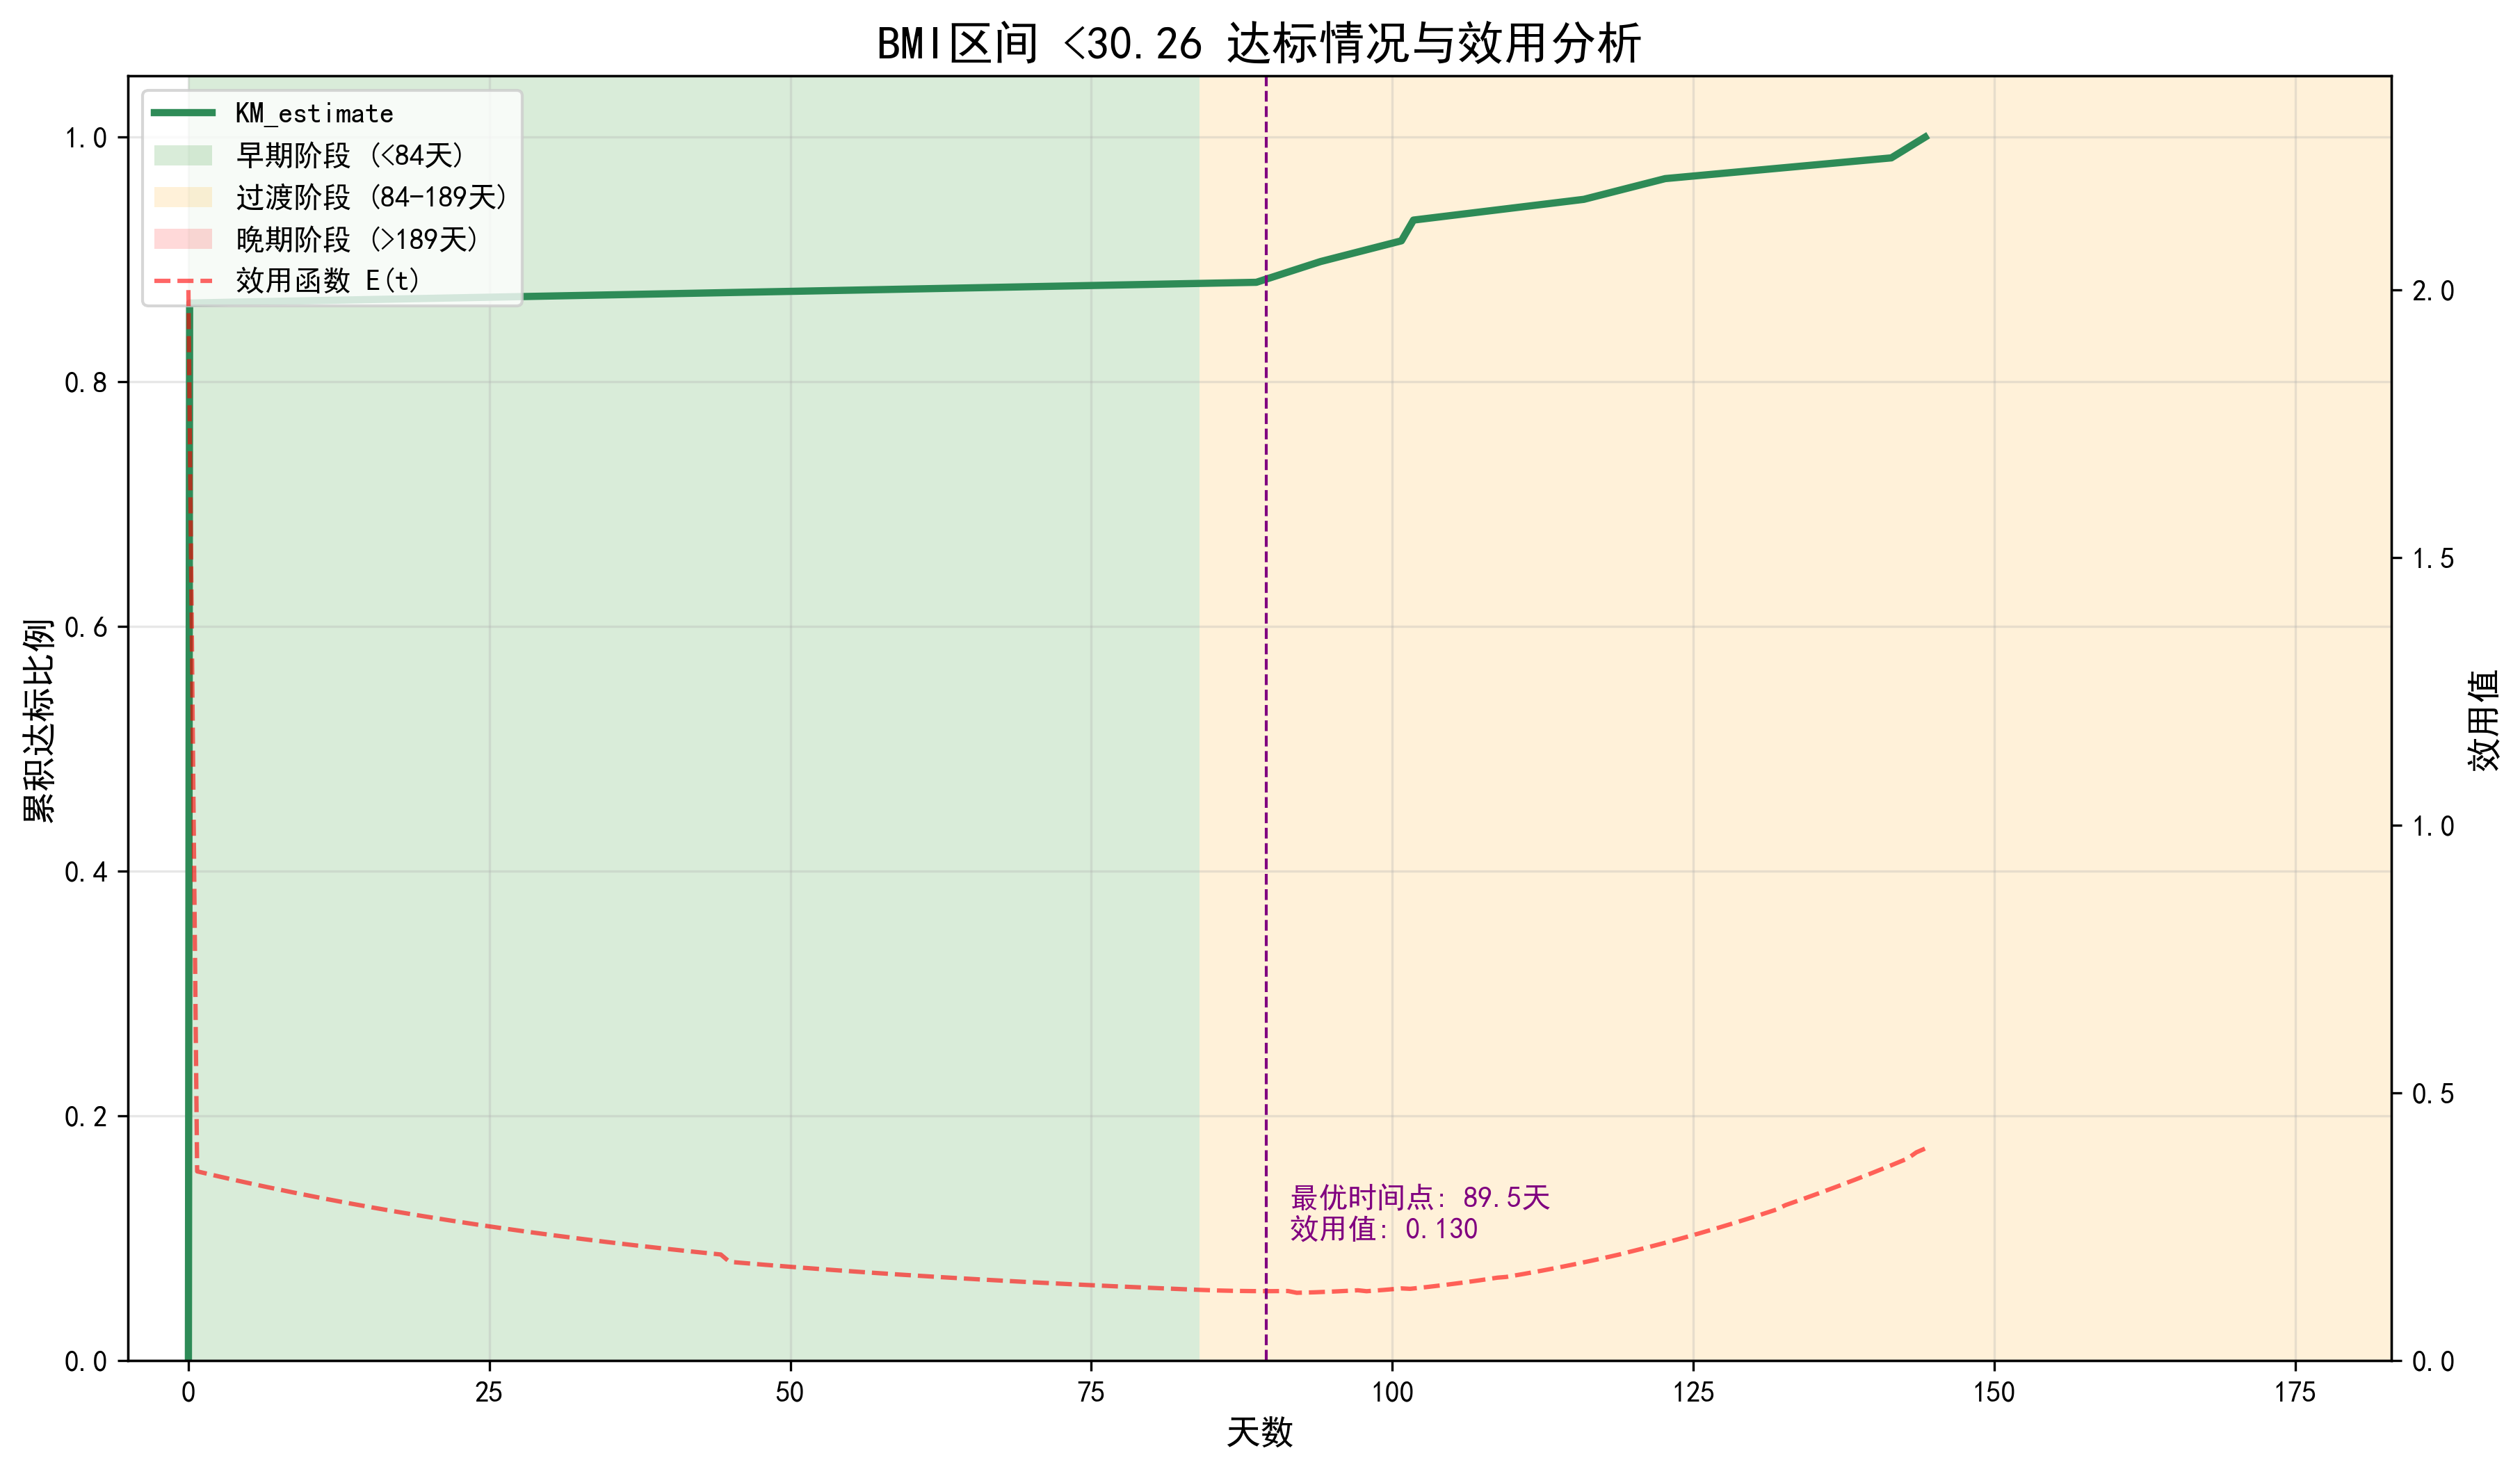
\includegraphics[width=\textwidth]{graph/BMI_lt30.26_utility_analysis.png}  % 宽度=子图宽度
        \caption{小于30.26组}  % 子标题
        \label{fig:sub1}  % 子图标签
    \end{subfigure}
    \hspace{0.05\textwidth}  % 两图间距(5%页面宽度)
    % 子图2
    \begin{subfigure}[b]{0.45\textwidth}
        \centering
        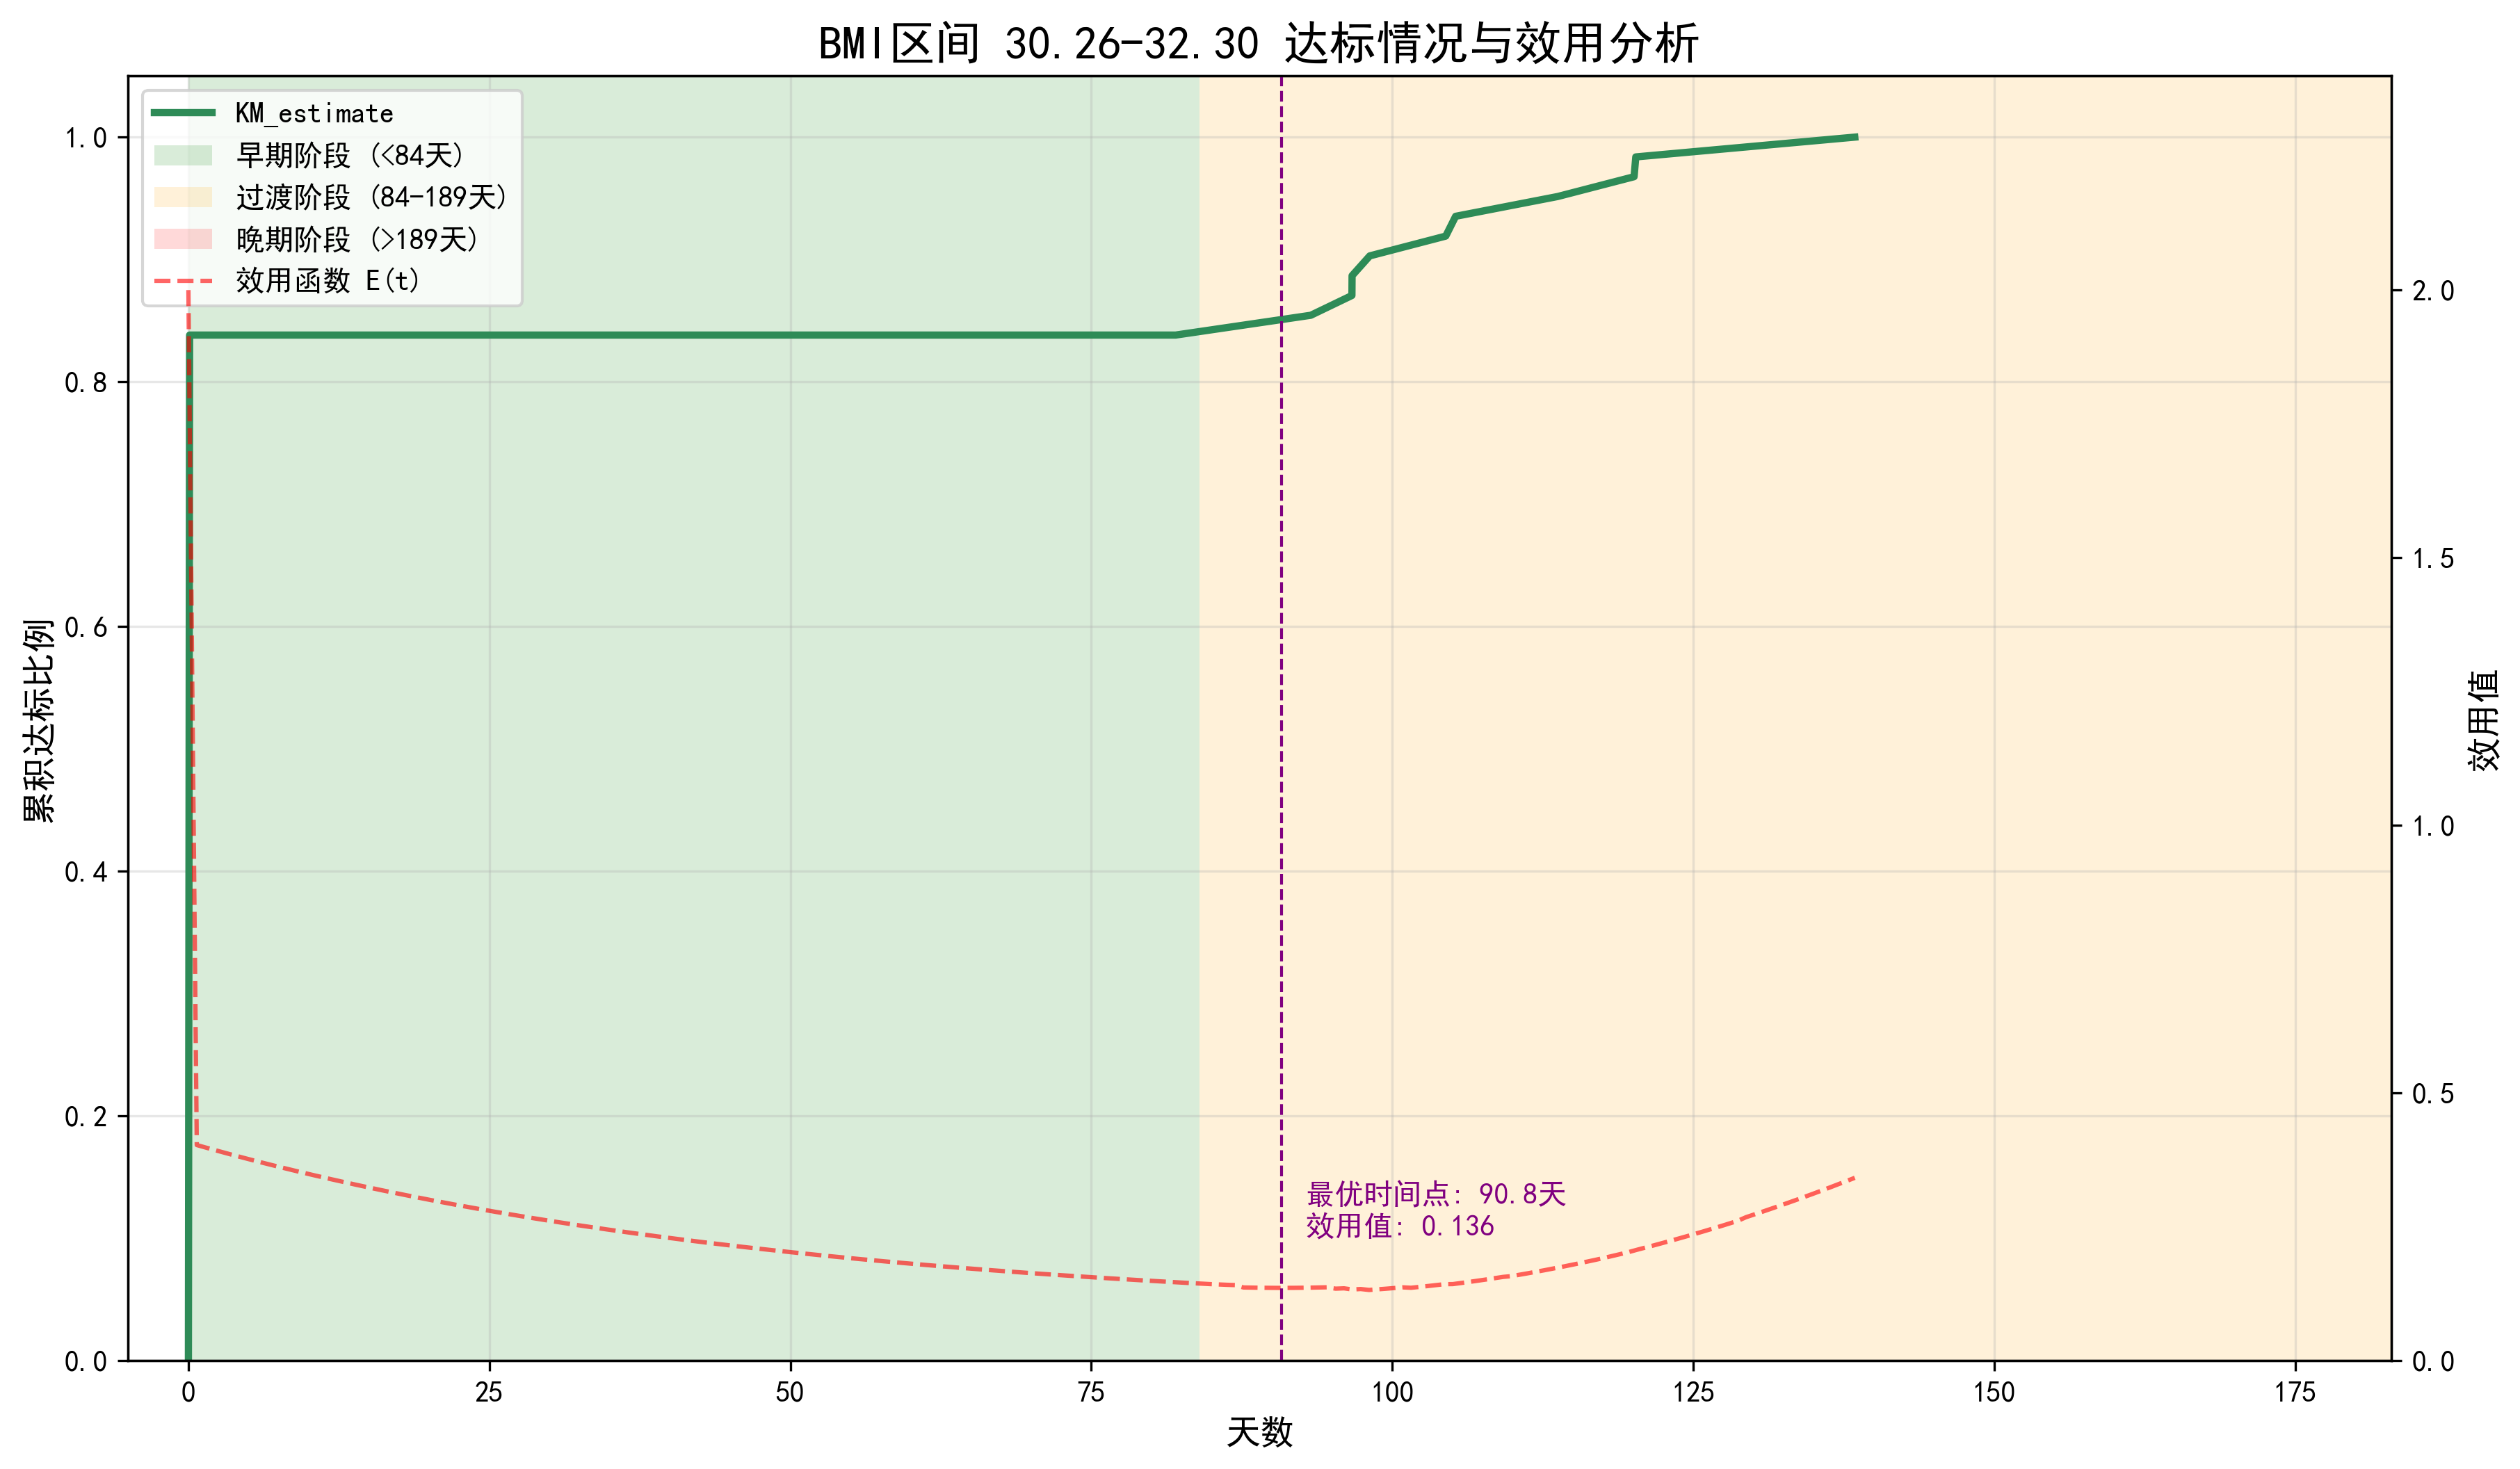
\includegraphics[width=\textwidth]{graph/BMI_30.26_32.30_utility_analysis.png}
        \caption{30.26-32.30组}
        \label{fig:sub2}
    \end{subfigure}
    \label{fig:two}  % 整体标签
\end{figure}
\begin{figure}[H]
    \centering
    % 子图1:宽度占页面的45%(左右留空)
    \begin{subfigure}[b]{0.45\textwidth}  % [b]表示底部对齐
        \centering
        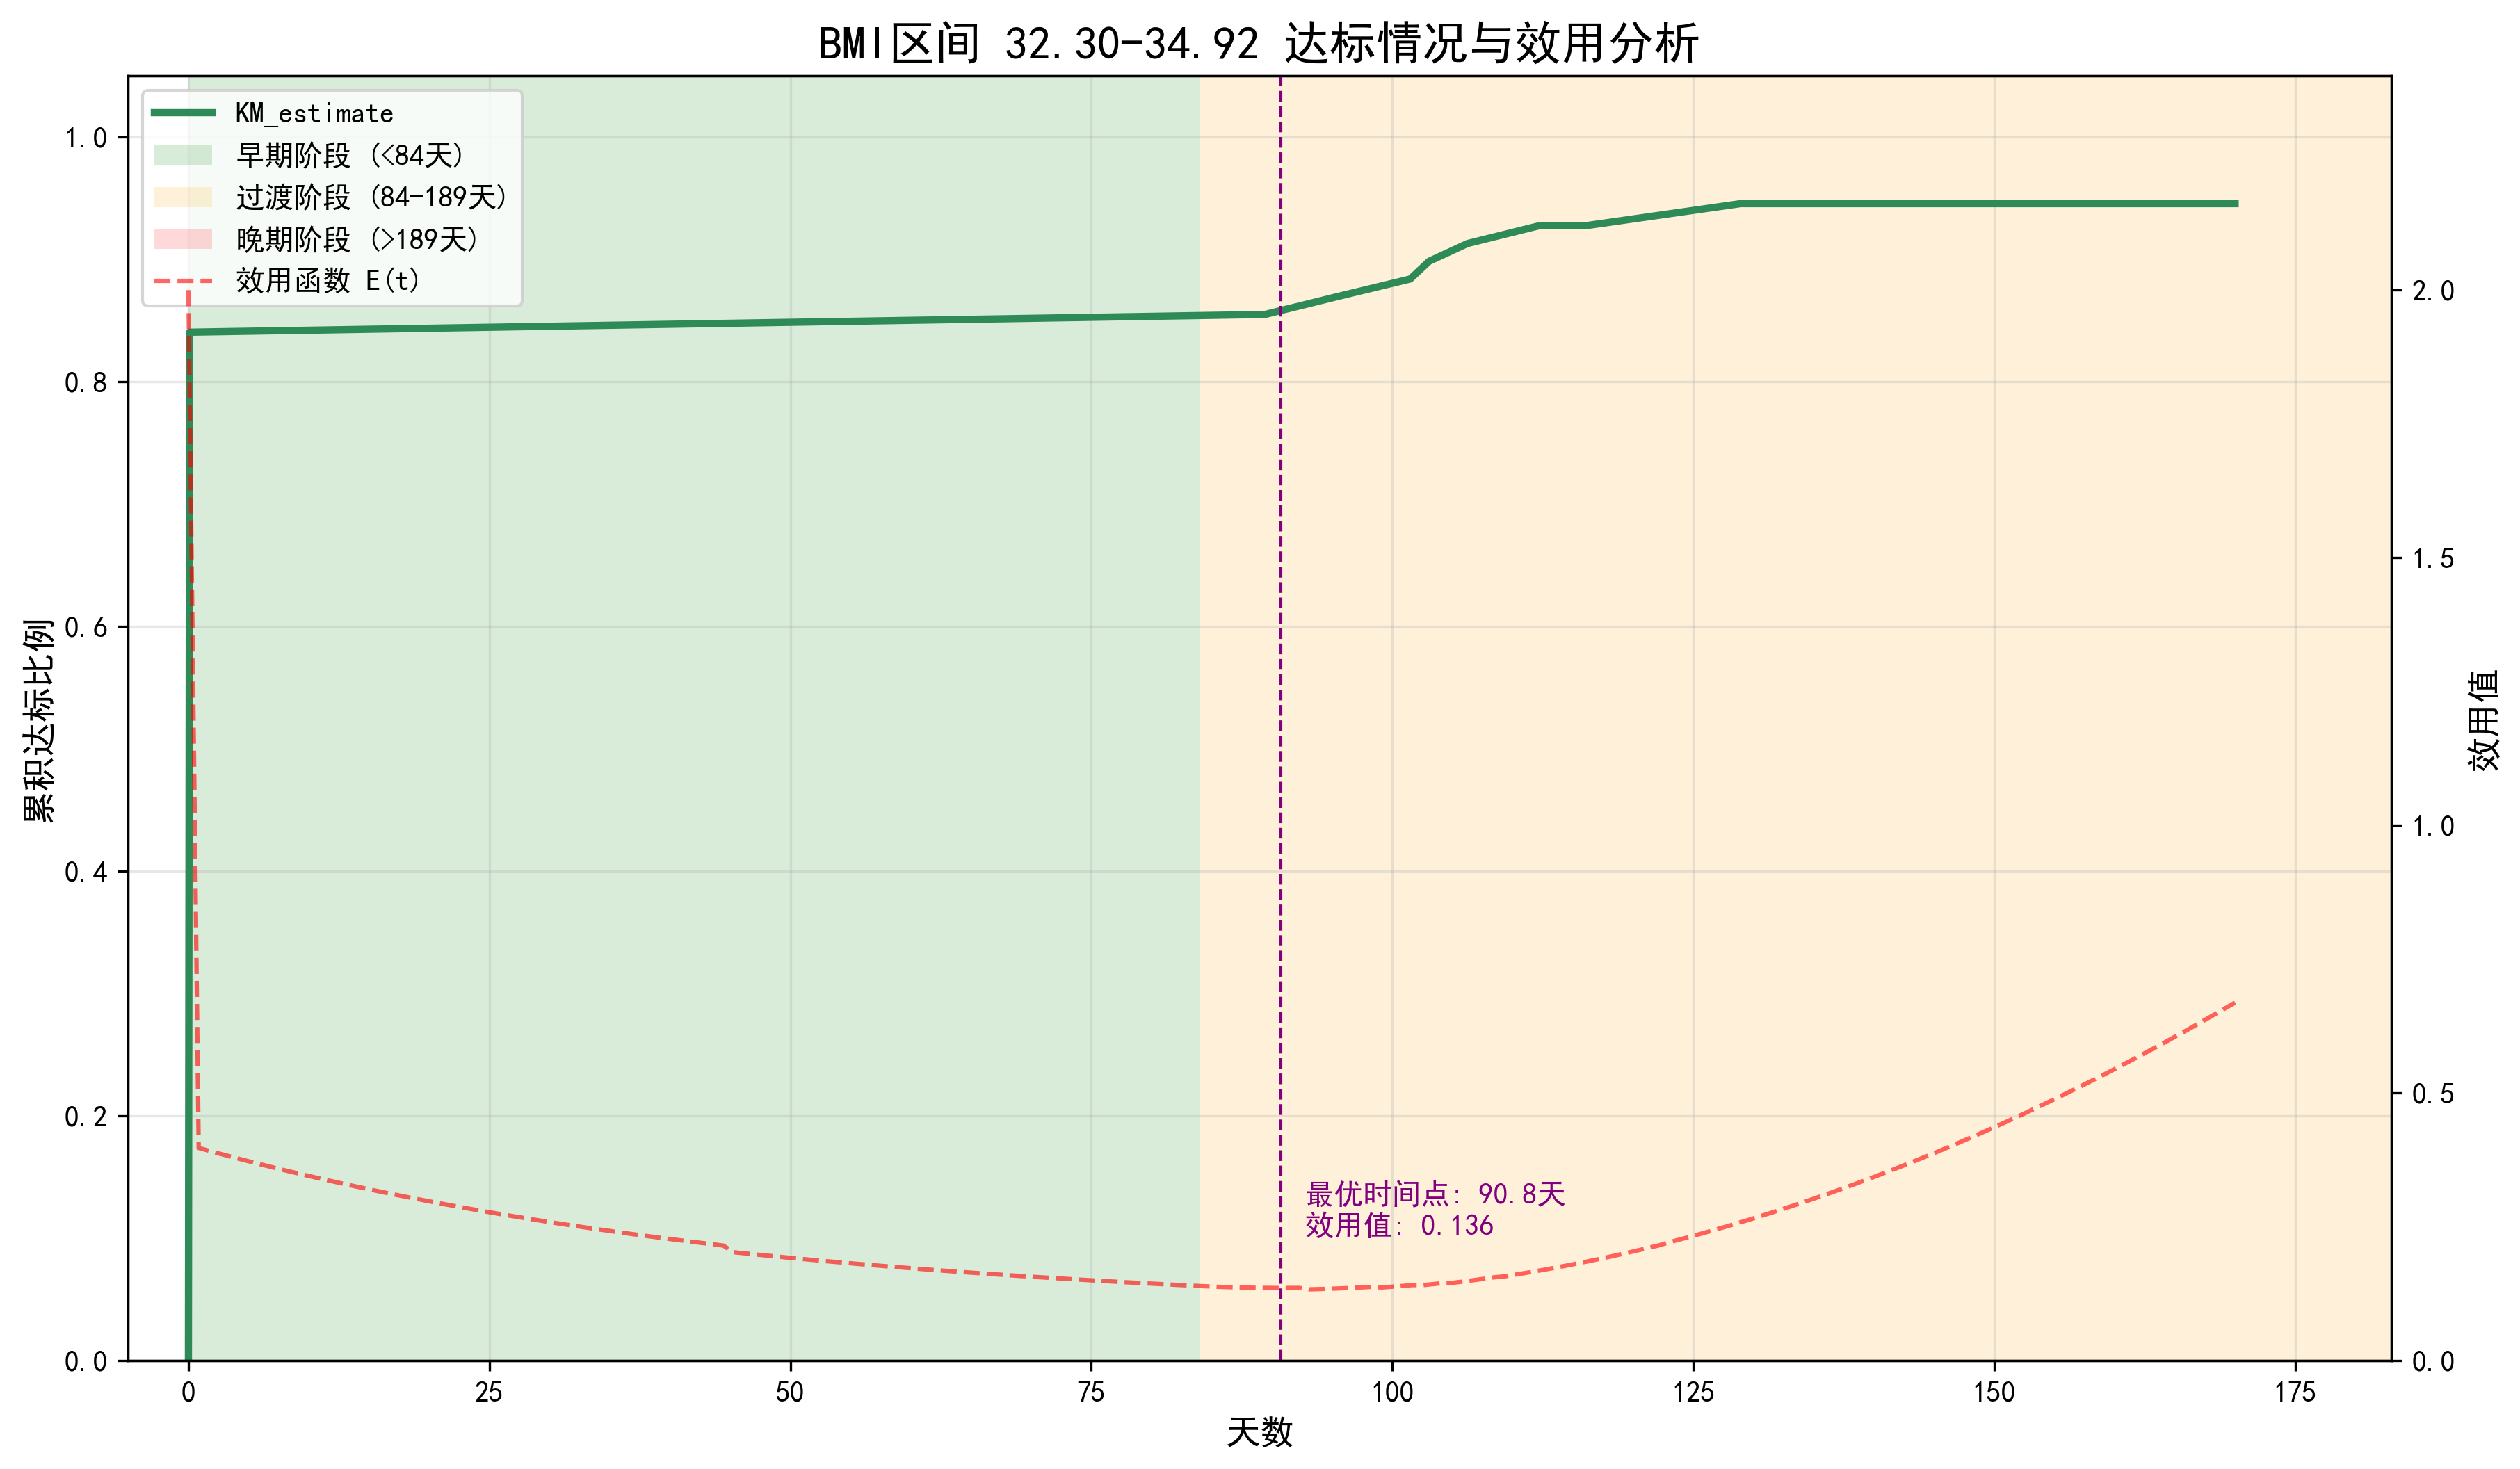
\includegraphics[width=\textwidth]{graph/BMI_32.30_34.92_utility_analysis.png}  % 宽度=子图宽度
        \caption{32.30-34.92组}  % 子标题
        \label{fig:sub1}  % 子图标签
    \end{subfigure}
    \hspace{0.05\textwidth}  % 两图间距(5%页面宽度)
    % 子图2
    \begin{subfigure}[b]{0.45\textwidth}
        \centering
        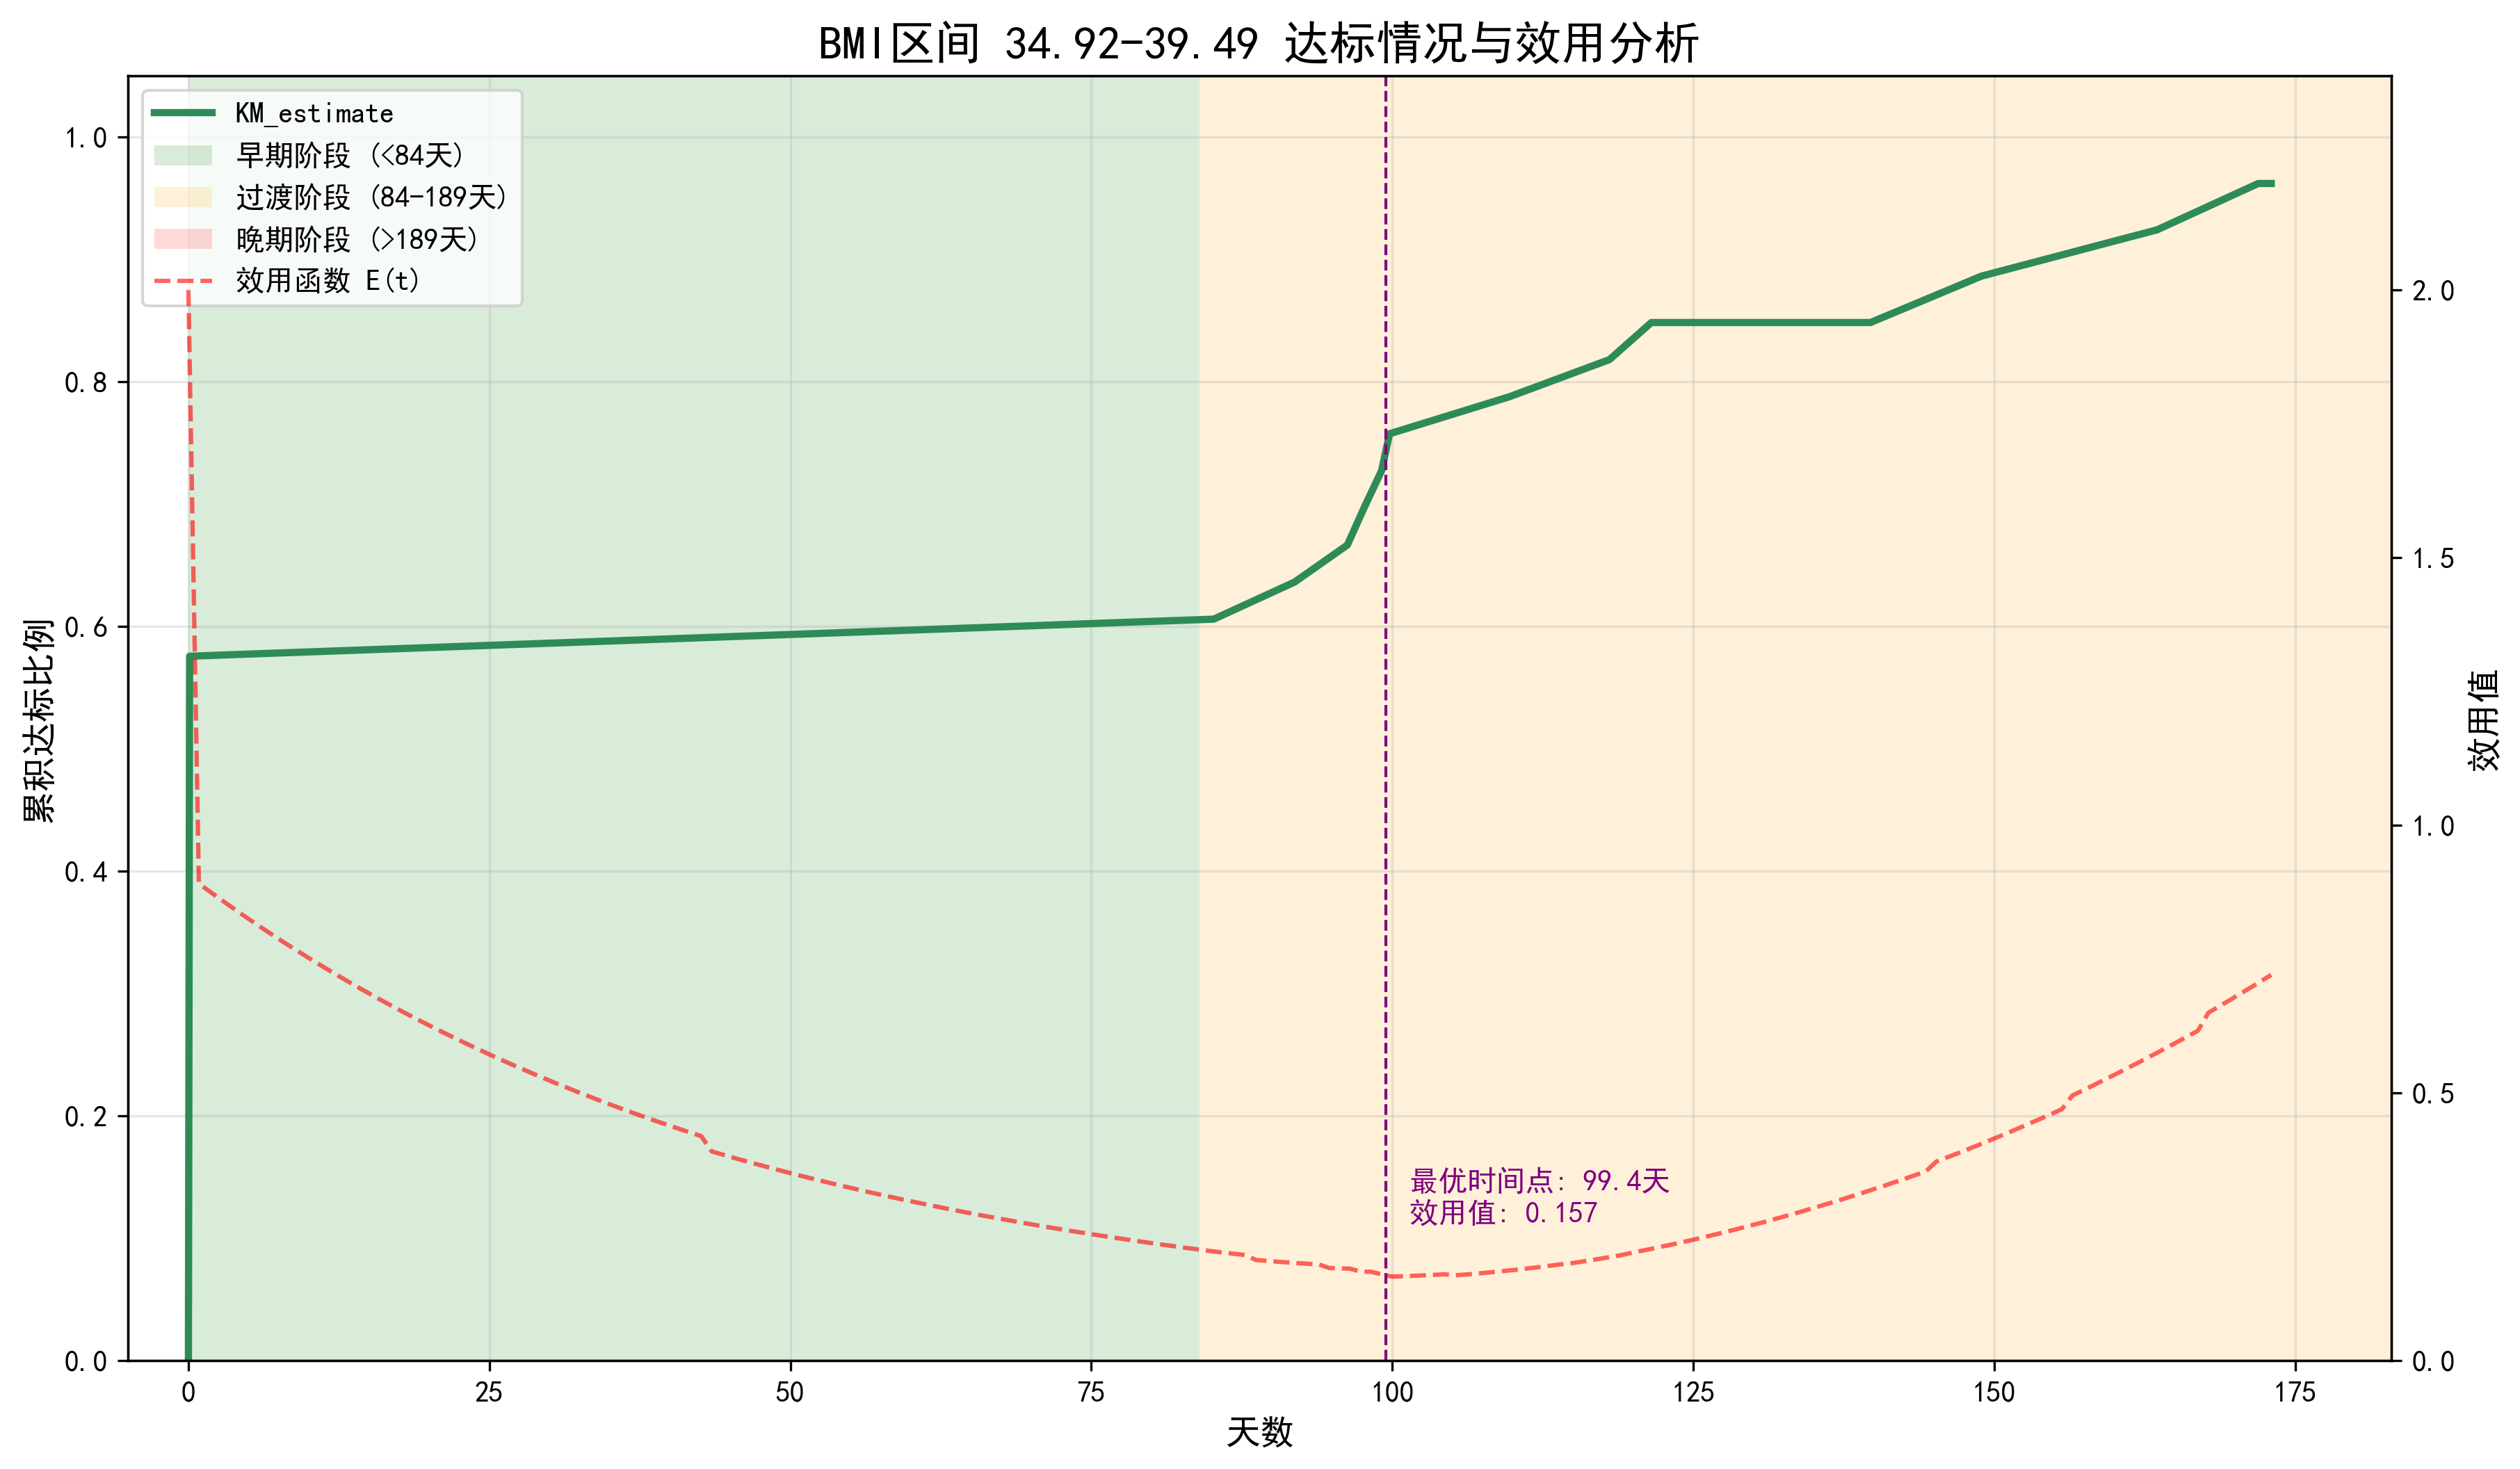
\includegraphics[width=\textwidth]{graph/BMI_34.92_39.49_utility_analysis.png}
        \caption{34.92-39.49组}
        \label{fig:sub2}
    \end{subfigure}
    \label{fig:two}  % 整体标签
\end{figure}

\begin{figure}[H]
    \centering
    % 子图1:宽度占页面的45%(左右留空)
    \begin{subfigure}[b]{0.45\textwidth}  % [b]表示底部对齐
        \centering
        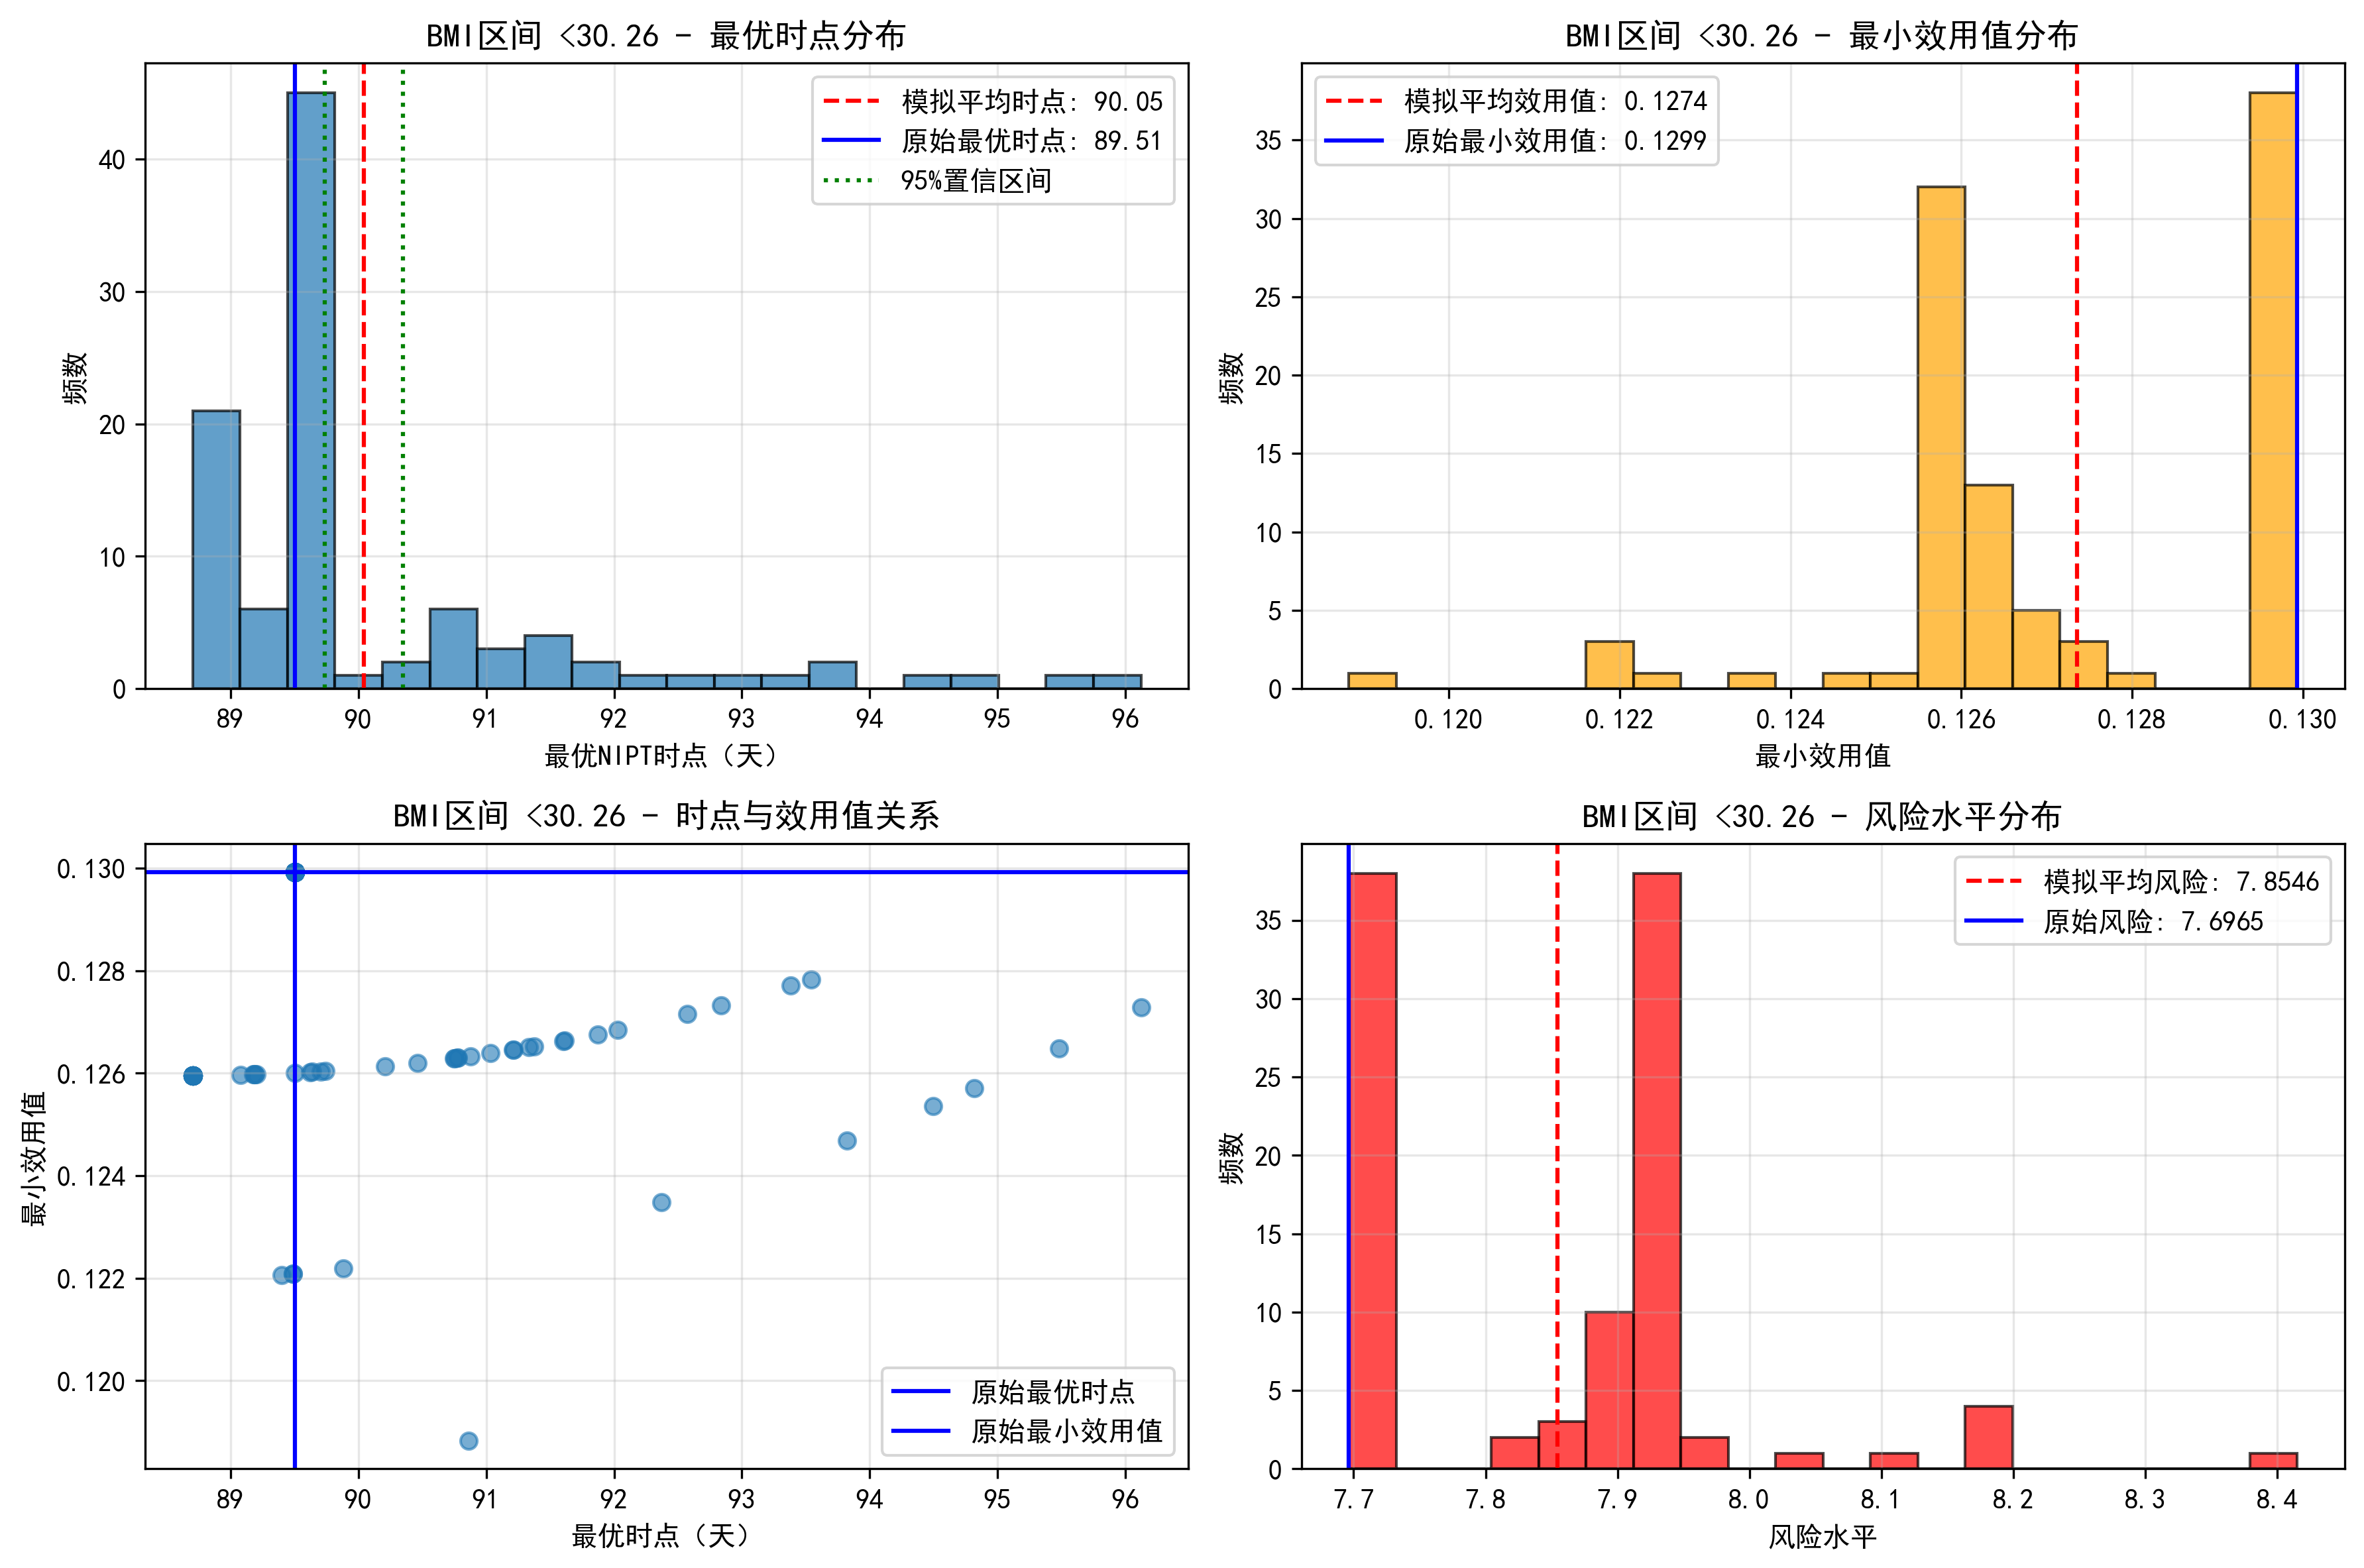
\includegraphics[width=\textwidth]{graph/error_analysis_BMI__30.26.png}  % 宽度=子图宽度
        \caption{小于30.26组}  % 子标题
        \label{fig:sub1}  % 子图标签
    \end{subfigure}
    \hspace{0.05\textwidth}  % 两图间距(5%页面宽度)
    % 子图2
    \begin{subfigure}[b]{0.45\textwidth}
        \centering
        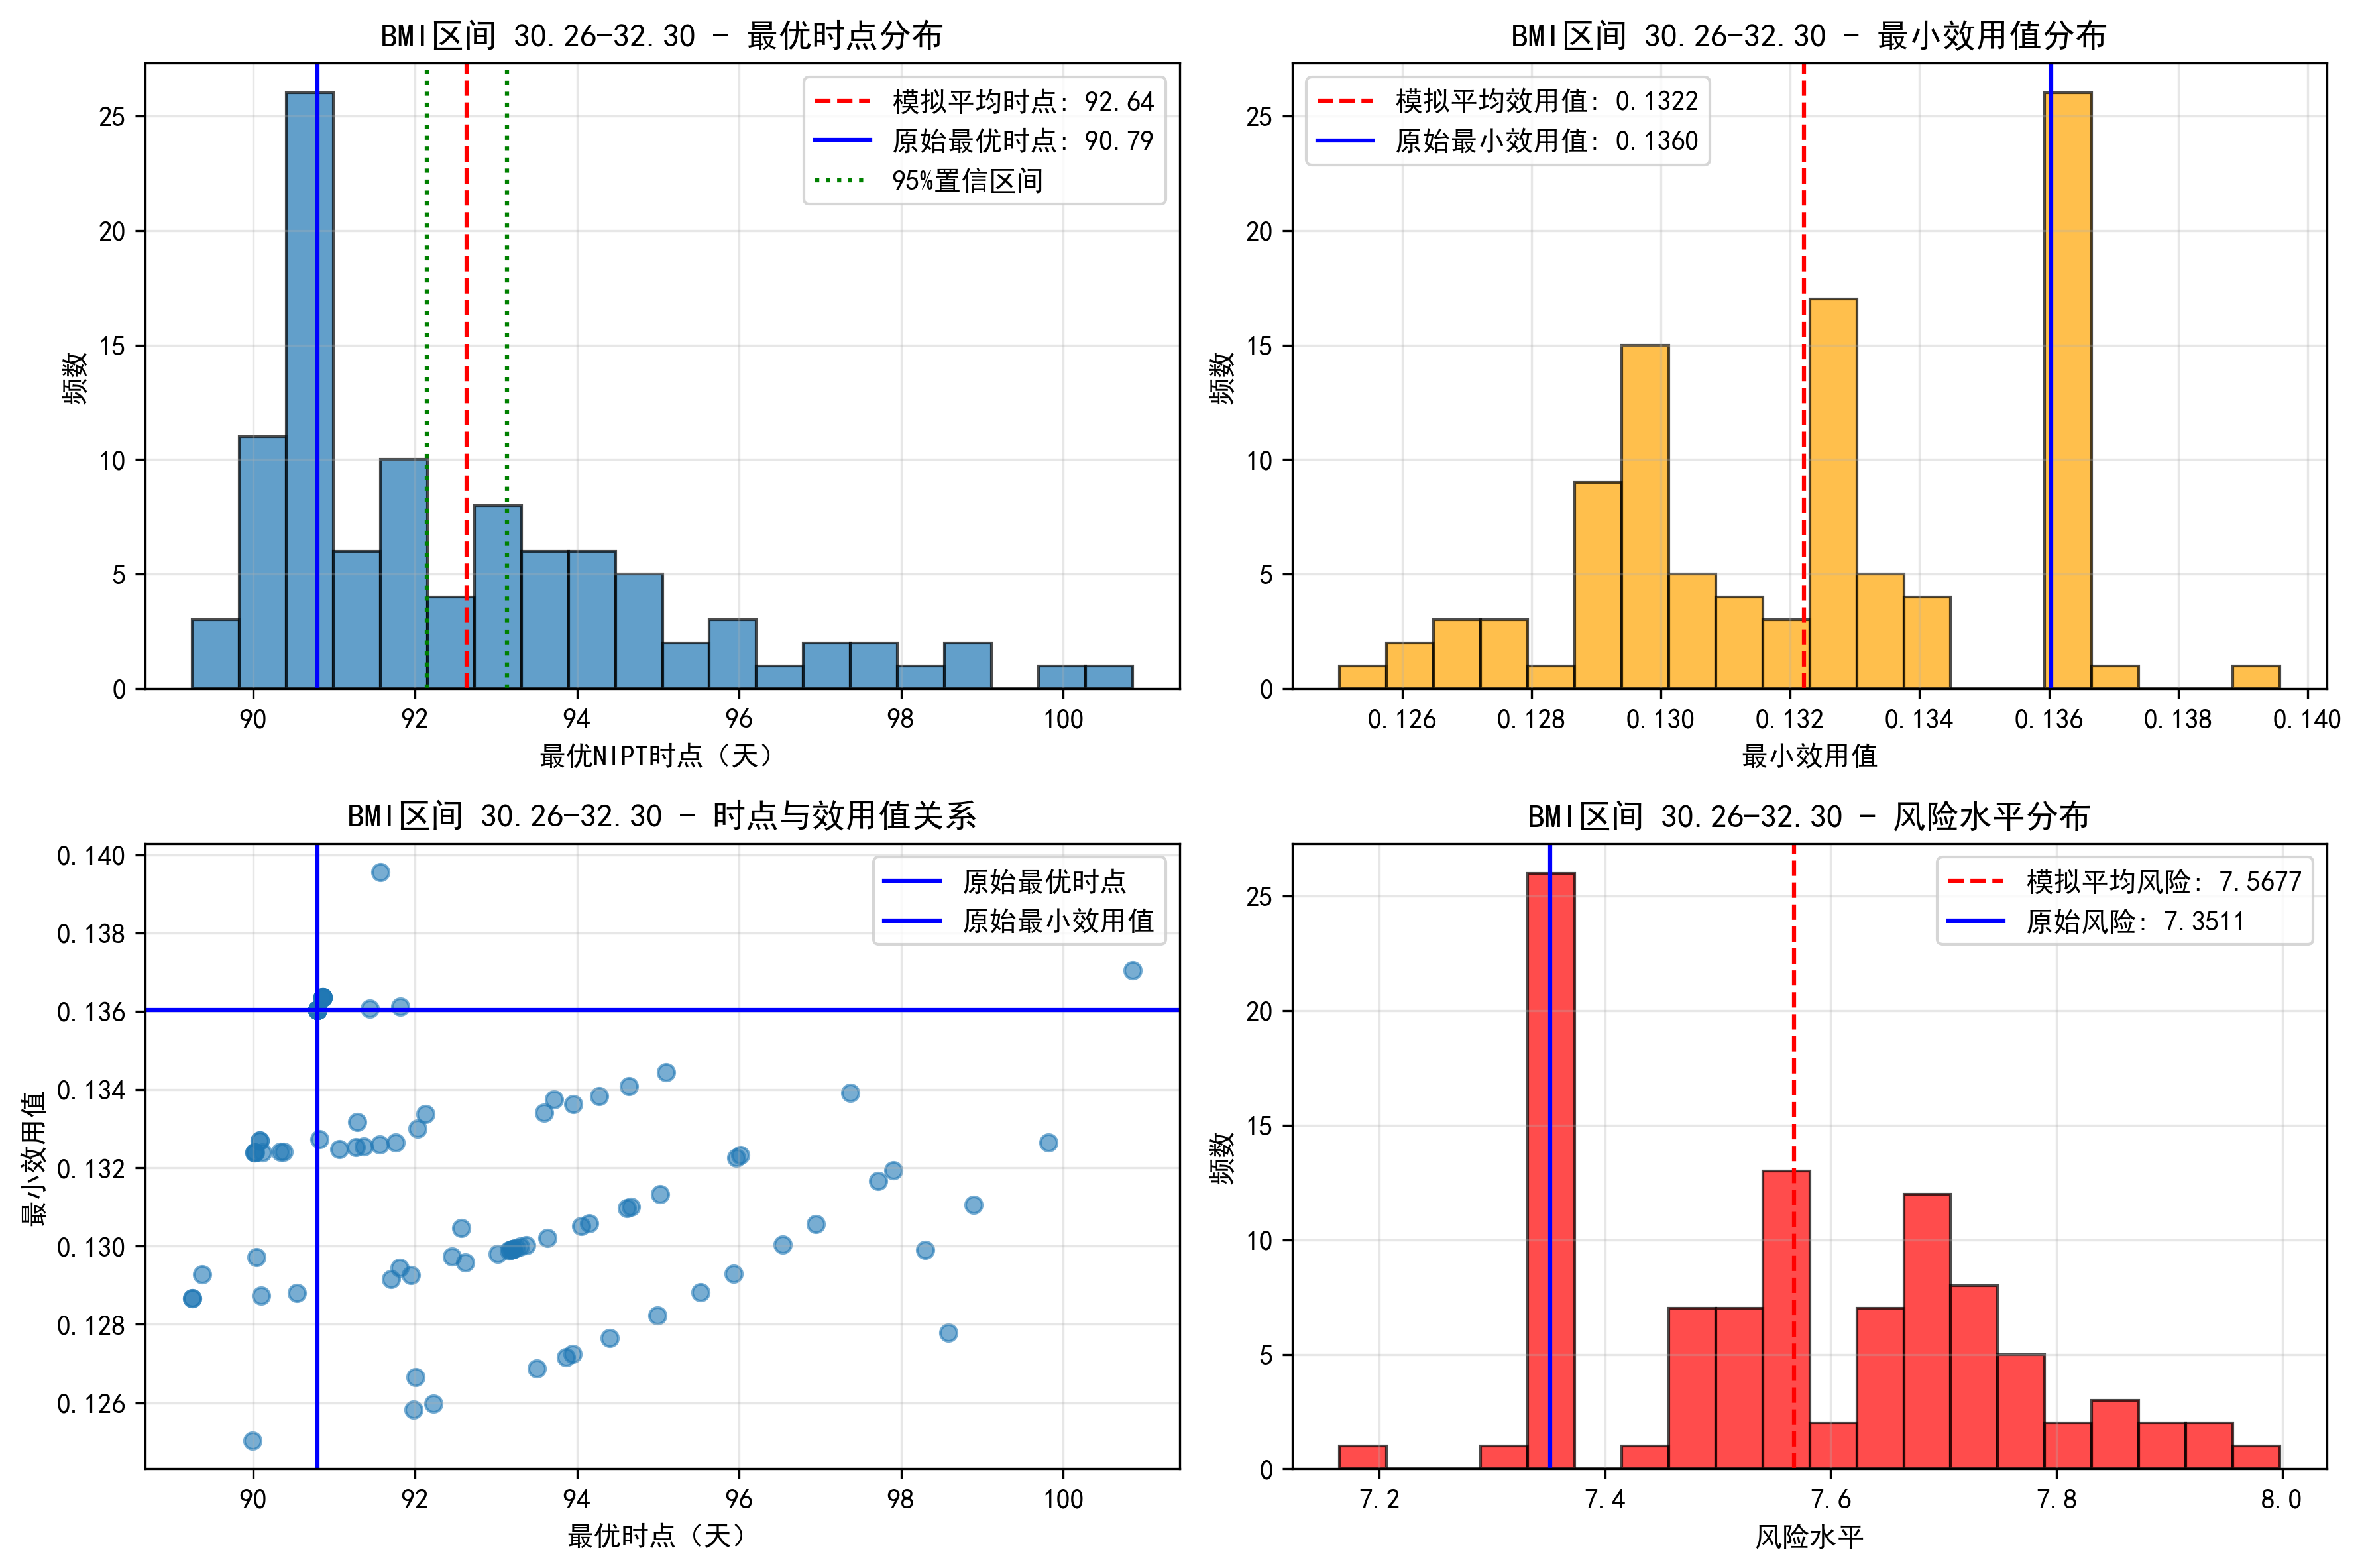
\includegraphics[width=\textwidth]{graph/error_analysis_BMI_30.26-32.30.png}
        \caption{30.26-32.30组}
        \label{fig:sub2}
    \end{subfigure}
    \label{fig:two}  % 整体标签
\end{figure}
\begin{figure}[H]
    \centering
    % 子图1:宽度占页面的45%(左右留空)
    \begin{subfigure}[b]{0.45\textwidth}  % [b]表示底部对齐
        \centering
        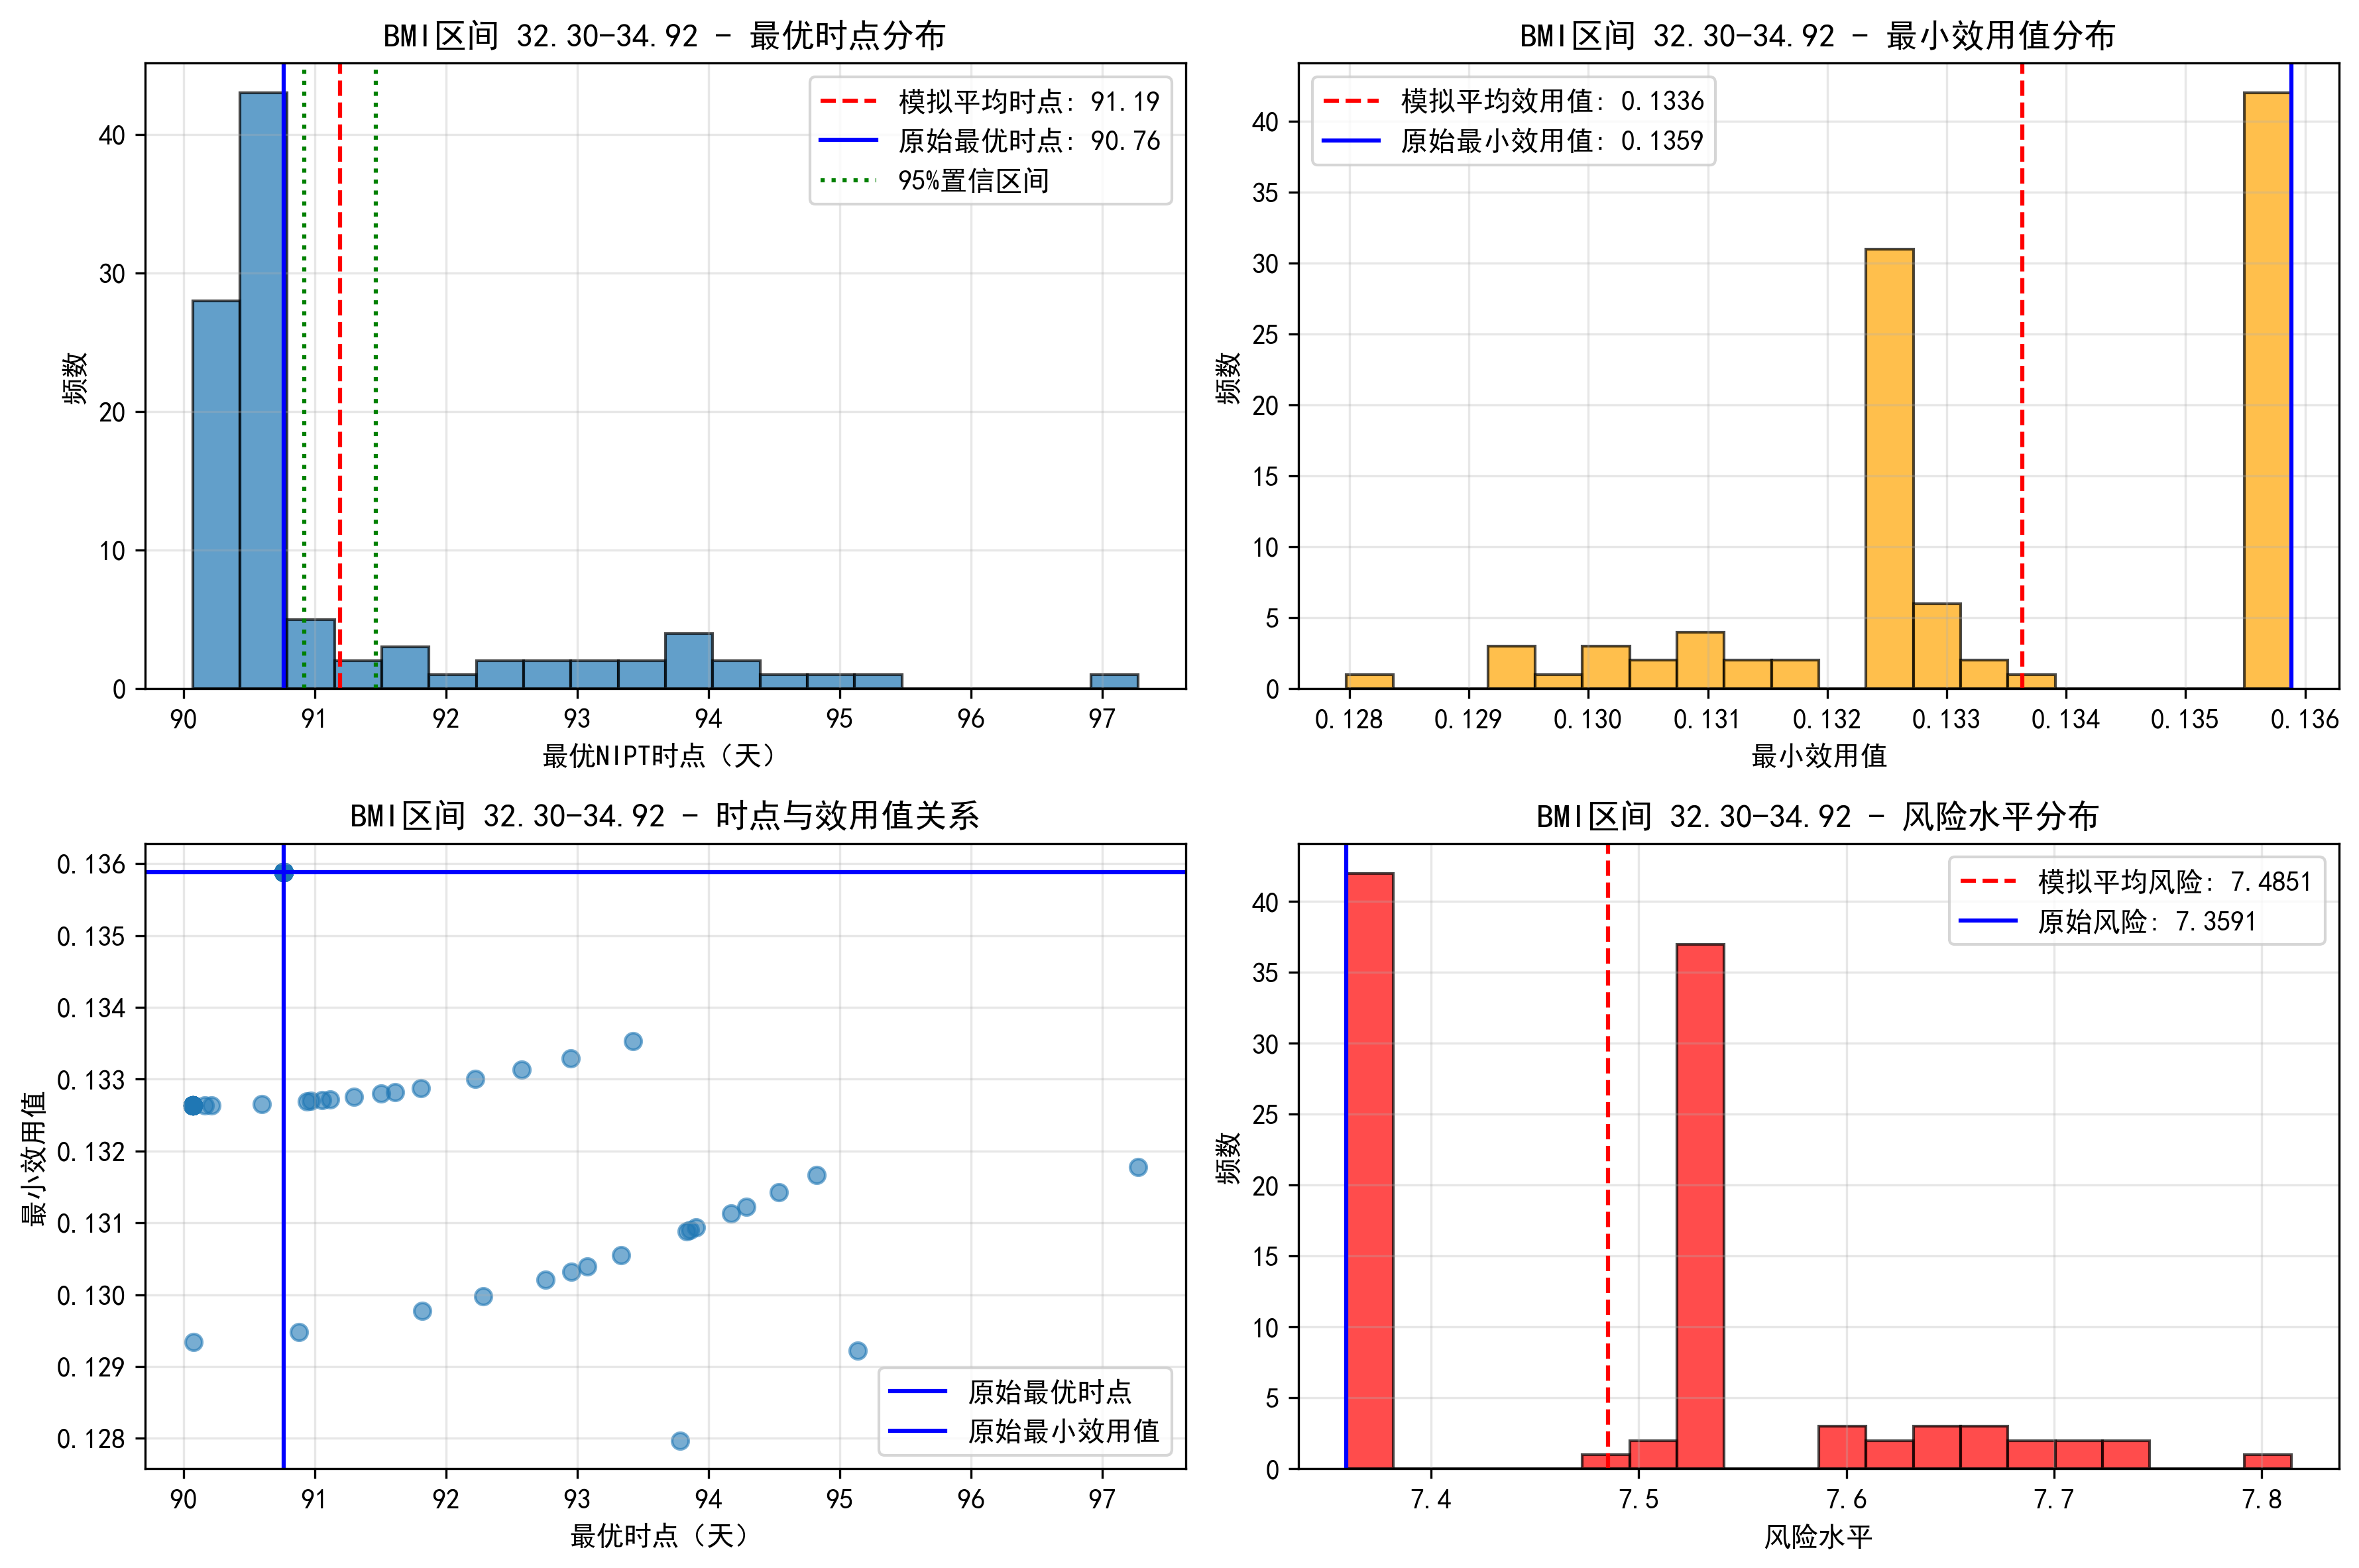
\includegraphics[width=\textwidth]{graph/error_analysis_BMI_32.30-34.92.png}  % 宽度=子图宽度
        \caption{32.30-34.92组}  % 子标题
        \label{fig:sub1}  % 子图标签
    \end{subfigure}
    \hspace{0.05\textwidth}  % 两图间距(5%页面宽度)
    % 子图2
    \begin{subfigure}[b]{0.45\textwidth}
        \centering
        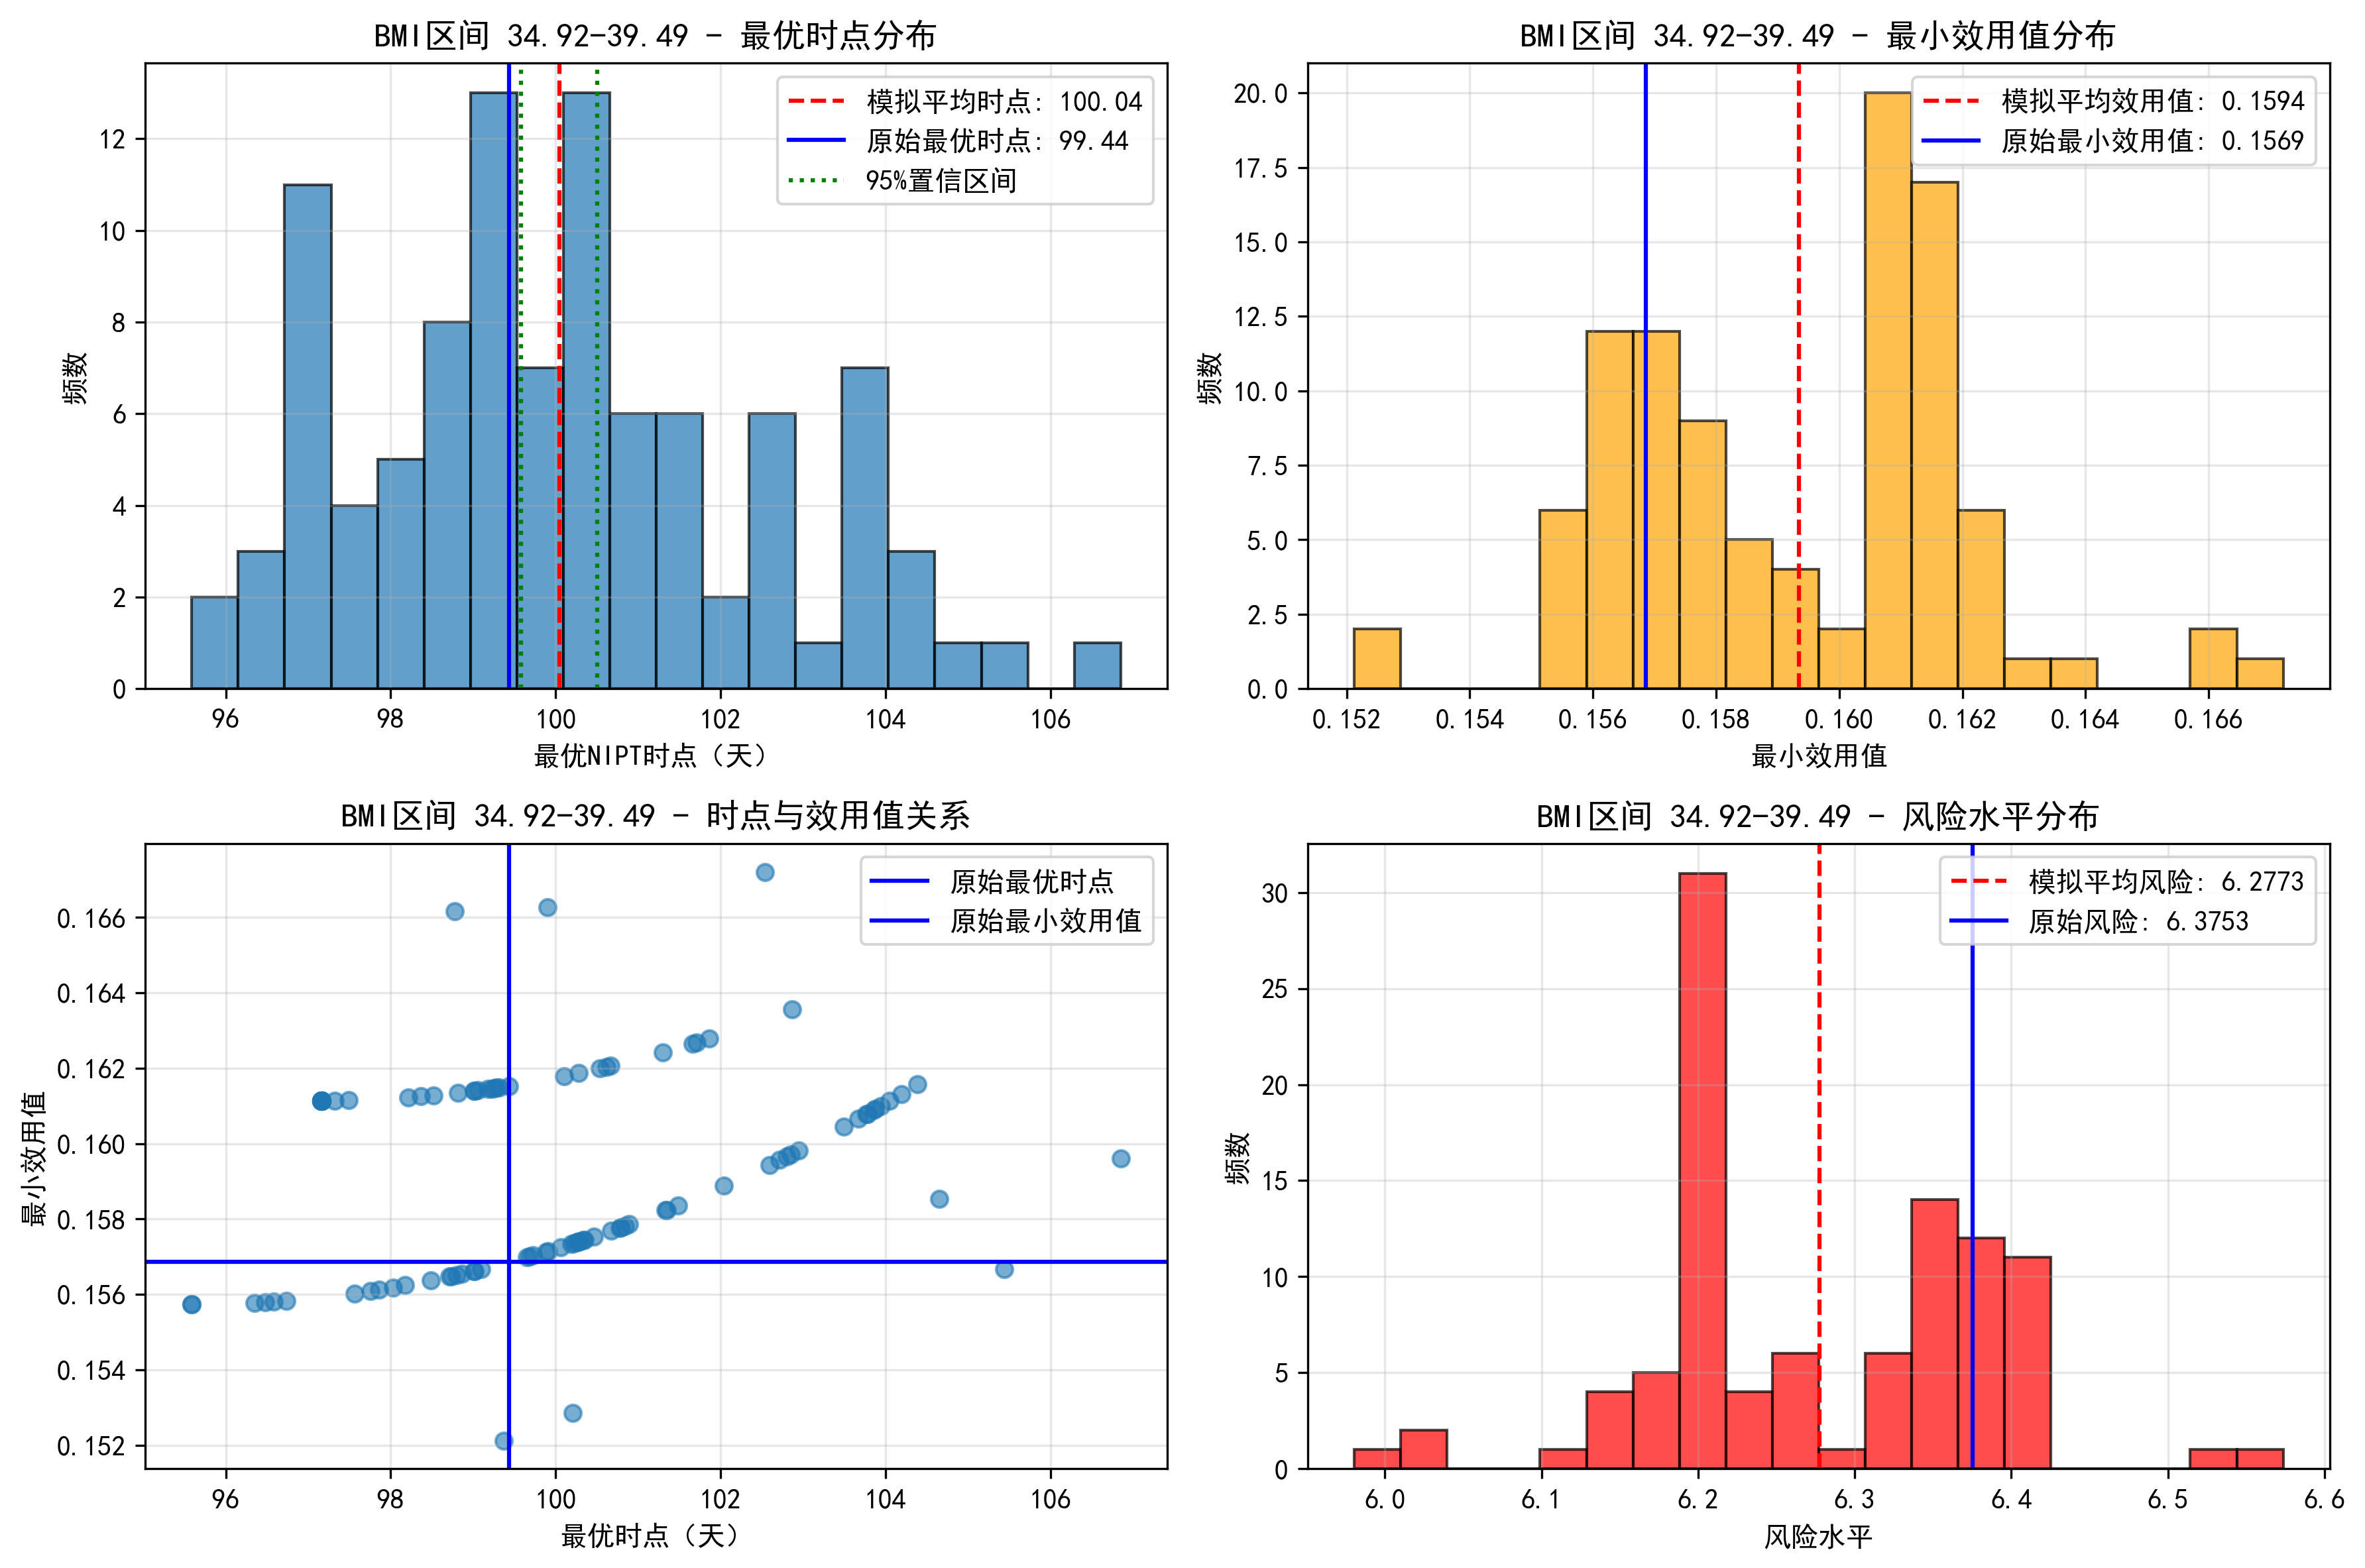
\includegraphics[width=\textwidth]{graph/error_analysis_BMI_34.92-39.49.png}
        \caption{34.92-39.49组}
        \label{fig:sub2}
    \end{subfigure}
    \label{fig:two}  % 整体标签
\end{figure}
% 单个图片
\end{comment}
